\section{Descripción del grupo}

\subsection{Grupo encuestado}

En Abril de 2021 lanzamos una convocatoria en la que le pedimos a docentes de escuelas argentinas que estuvieran dando clases a alumnos de alrededor de 10 años que nos contactaran para colaborar en la actividad.

Logramos coordinar con una docente de una escuela pública de Rosario, Santa Fé para que participara junto con sus alumnos de 4to y 5to grado, siendo en total 144 niños y niñas.

Ese mismo mes y a lo largo de dos semanas, en la medida que la docente tenía clases con estos cursos, fue proponiéndoles que completen la encuesta y de esta forma fuimos recibiendo sus respuestas. 

Las respuestas recibidas en días posteriores no fueron tenidas en cuenta, ya que no teníamos certeza de que las respuestas reflejaran el conocimiento o las concepciones de los chicos (podría pasar que, al contestar por fuera del marco de la clase, no cumplieran la consigna de no buscar información en Internet o preguntar a otras personas).

Cabe destacar que, en el momento en el que se realizó la convocatoria, en Argentina se estaba transicionando de una vuelta a la presencialidad a el dictado de clases de manera online, por lo que muchas escuelas se encontraban organizándose frente a este cambio y no tenían disponibilidad para realizar la actividad con sus alumnos. Por este motivo, no nos fue posible conseguir otras escuelas que pudieran participar.

\subsection{Análisis Poblacional}

A continuación se describe el grupo encuestado según distintas variables poblacionales. 

\begin{figure}[h]
    \centering
    \begin{minipage}{0.50\textwidth}
        \centering
        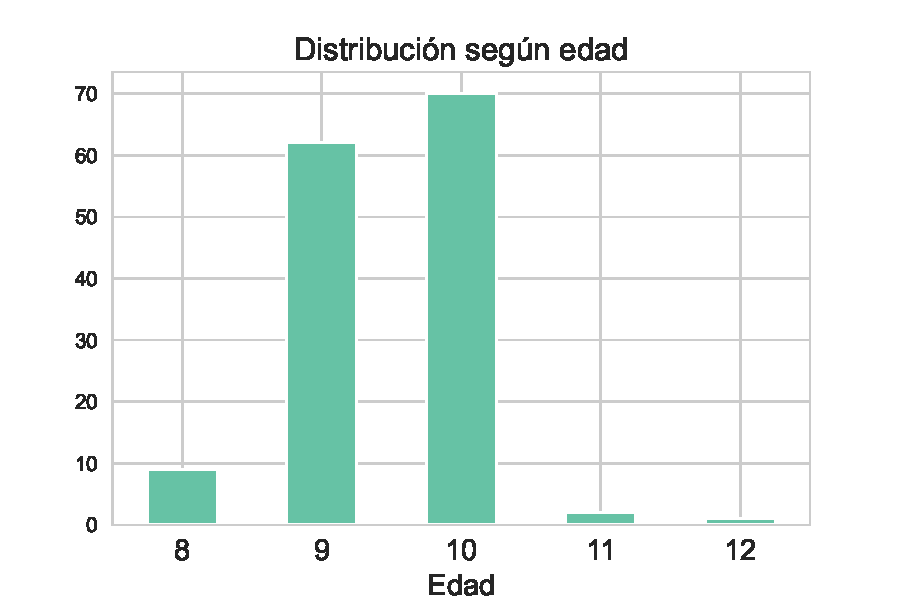
\includegraphics[width=0.9\textwidth]{images_analisis/1.pdf} 
        \caption{Participantes distribuidos por edad.}
        \label{fig:analisis1}
    \end{minipage}\hfill
    \begin{minipage}{0.50\textwidth}
        \centering
        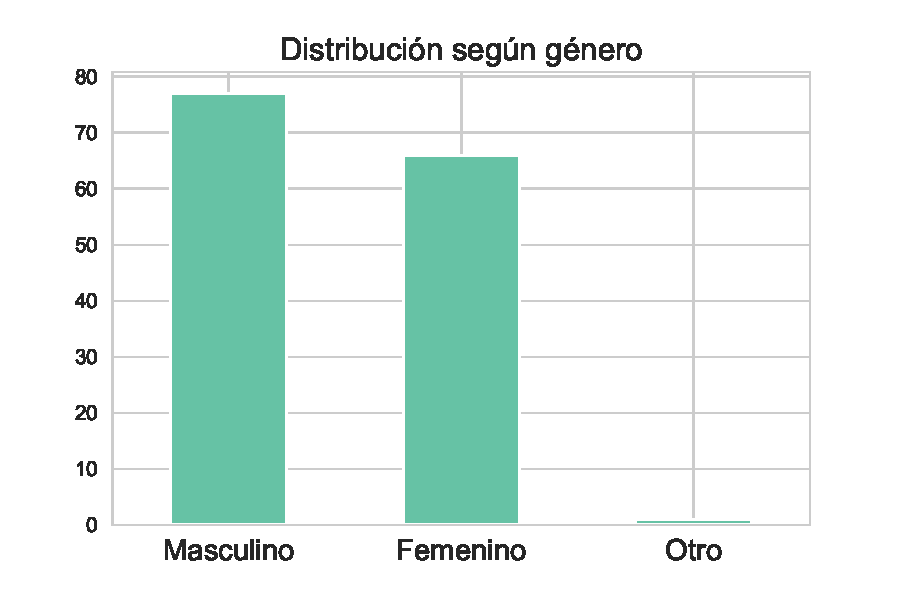
\includegraphics[width=0.9\textwidth]{images_analisis/2.pdf} 
        \caption{Participantes distribuidos por género}
        \label{fig:analisis2}
    \end{minipage}
\end{figure}

Podemos ver en la Fig. \ref{fig:analisis1} que se trata de un grupo bastante homogéneo en cuanto a la edad, en tanto es el objeto de nuestro estudio el grupo comprendido por niños y niñas de alrededor de diez años. En cuanto al género, observamos en la Fig. \ref{fig:analisis2} que tenemos también una distribución muy pareja.

Tras analizar la Fig. \ref{fig:analisis3} nos queda claro que la mayor parte de los participantes utilizan la computadora en su casa. Siendo que tanto este año como el anterior vivimos en un contexto de pandemia, este resultado no resulta sorprendente.

Podemos destacar que la mayoría parecieran contar con una computadora en sus hogares, siendo tan solo uno de ellos quien respondió que no poseía una.

También les preguntamos para qué utilizan más comúnmente la computadora. Les dimos la posibilidad de marcar más de una opción dentro de una serie de respuestas y, al mismo tiempo, dejamos un espacio disponible para poder completar con otras actividades que no estuvieran dentro de las que les habíamos propuesto.

\begin{figure}[h]
    \centering
    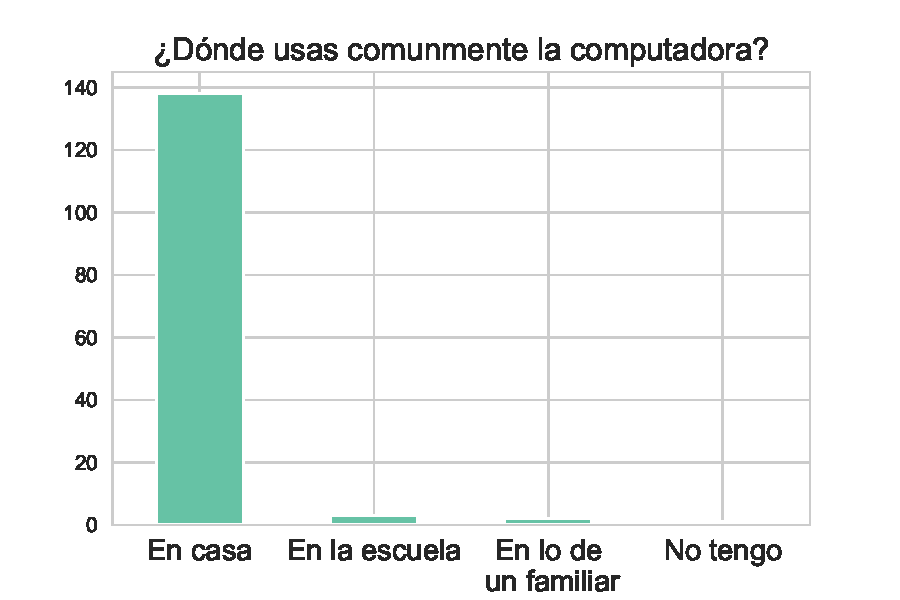
\includegraphics[width=0.5\textwidth]{images_analisis/3.pdf}
    \caption{Lugar en el que los participantes más usan la computadora.}
    \label{fig:analisis3}
\end{figure}

Es posible observar en la Fig. \ref{fig:analisis4} que la mayor parte de los encuestados utiliza la computadora para jugar juegos, siendo las siguientes actividades más usuales mirar videos en YouTube, realizar videollamadas utilizando Skype, Meet o Zoom, y realizar actividades escolares. Nuevamente, esto tiene sentido ya que durante todo el 2020 en Argentina hubo clases de manera virtual.

\begin{figure}[h]
    \centering
    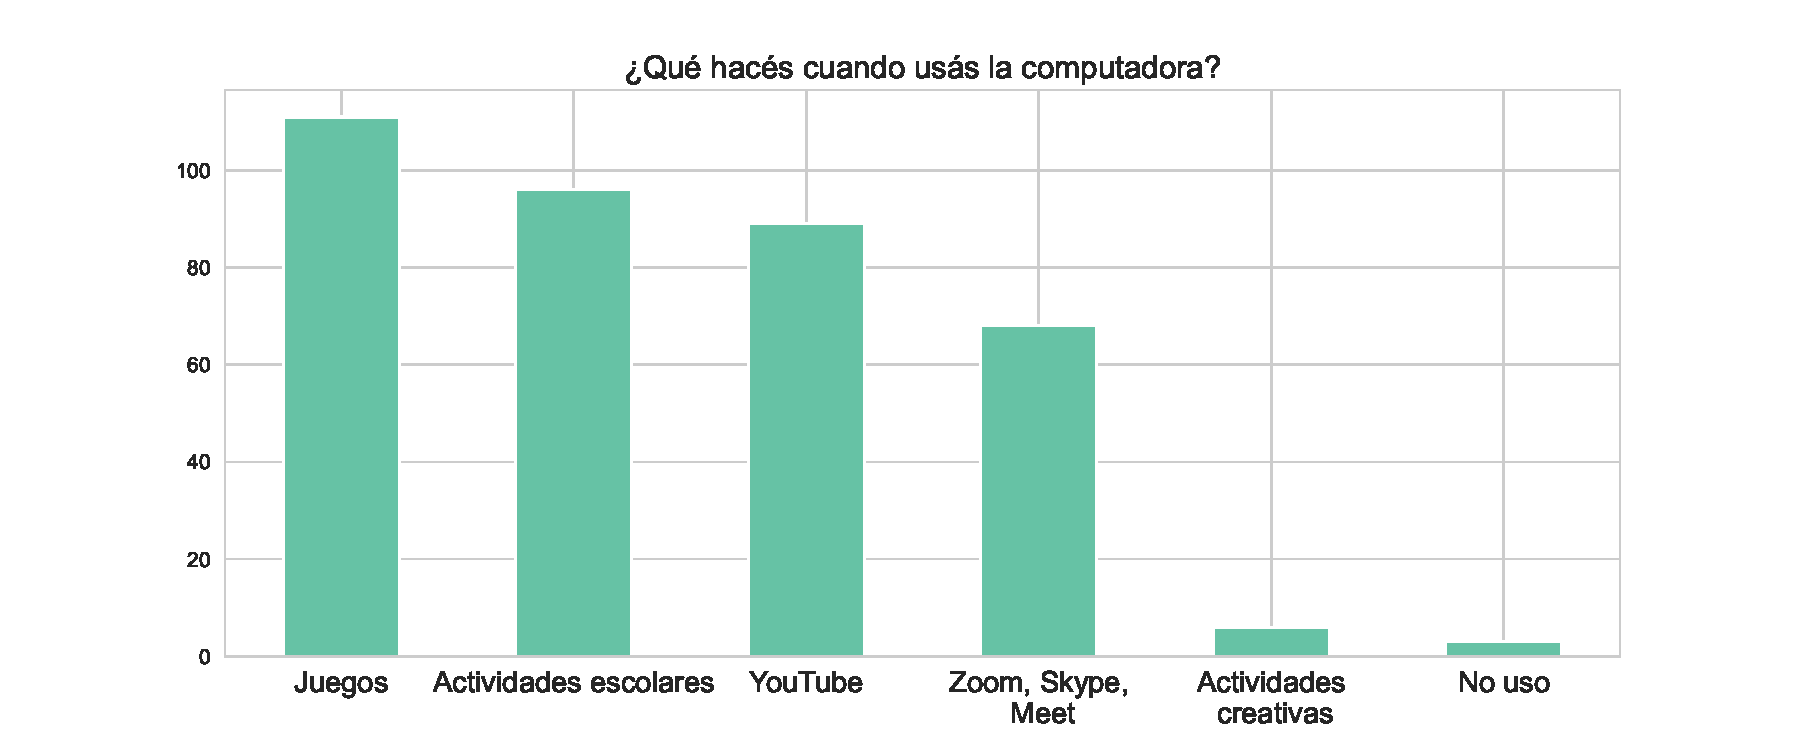
\includegraphics[width=1\textwidth]{images_analisis/4.pdf}
    \caption{Actividades más comunes al utilizar la computadora.}
    \label{fig:analisis4}
\end{figure}

\begin{figure}[h]
    \centering
    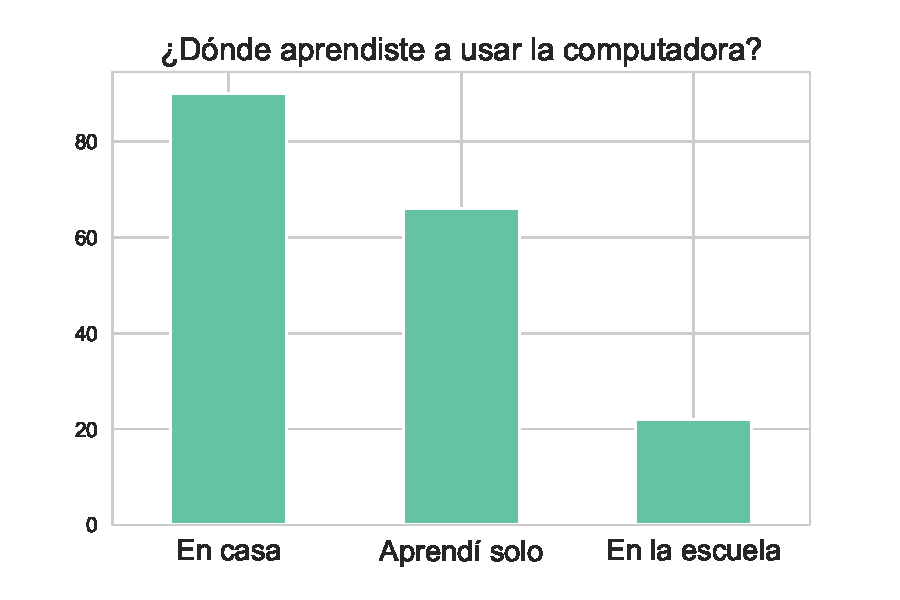
\includegraphics[width=0.50\textwidth]{images_analisis/5.pdf}
    \caption{Lugar o forma en la que aprendieron a utilizar la computadora.}
    \label{fig:analisis5}
\end{figure}

En cuanto a la forma en la que aprendieron a usar la computadora, se puede ver en la Fig. \ref{fig:analisis5} que las opciones más elegidas son ``\textit{Me enseñaron en mi casa (mis padres, hermanos u otro familiar)}'' y ``\textit{Aprendí solo}''.

Podemos ver que la tendencia está claramente más orientada a la formación recibida en el hogar, tanto por la enseñanza directa por parte de la familia o bien tal vez por la observación o la experiencia indirecta, al ver a otros miembros de la familia.

Esta hipótesis es respaldada por otros estudios anteriores, como por ejemplo el de Mertala \cite{mertala}, que explica que el conocimiento de los chicos sobre las distintas tecnologías se basa en el contacto que tuvieron con estas a través de sus padres, hermanos u otras figuras del entorno familiar o escolar.

De esta forma, esta percepción de haber ``aprendido solos'' podría tener raíz en este contacto indirecto.

Al indagar en la forma en que los chicos y chicas utilizan los celulares nos encontramos con que la gran mayoría cuenta con un dispositivo propio, como se puede observar en la Fig. \ref{fig:analisis6}.

\begin{figure}[h]
    \centering
    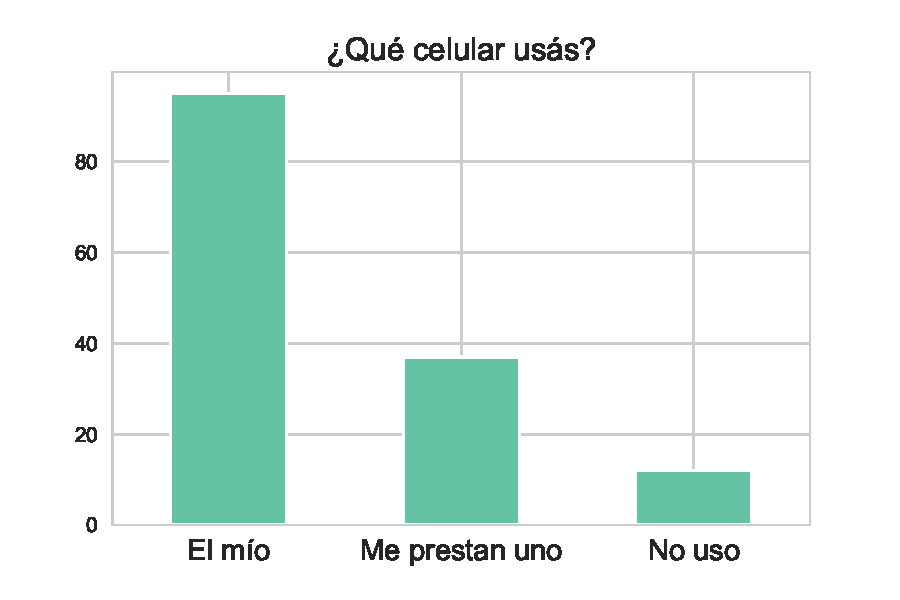
\includegraphics[width=0.6\textwidth]{images_analisis/6.pdf}
    \caption{Tipo de celular que utilizan (propio o prestado).}
    \label{fig:analisis6}
\end{figure}

En la Fig. \ref{fig:analisis7} vemos que la actividad más realizada es nuevamente jugar juegos, pero se suma con mucha importancia también el chat (utilizando aplicaciones de mensajería tales como Whatsapp, Telegram, etc.) y mirar videos en YouTube.

\begin{figure}[h]
    \centering
    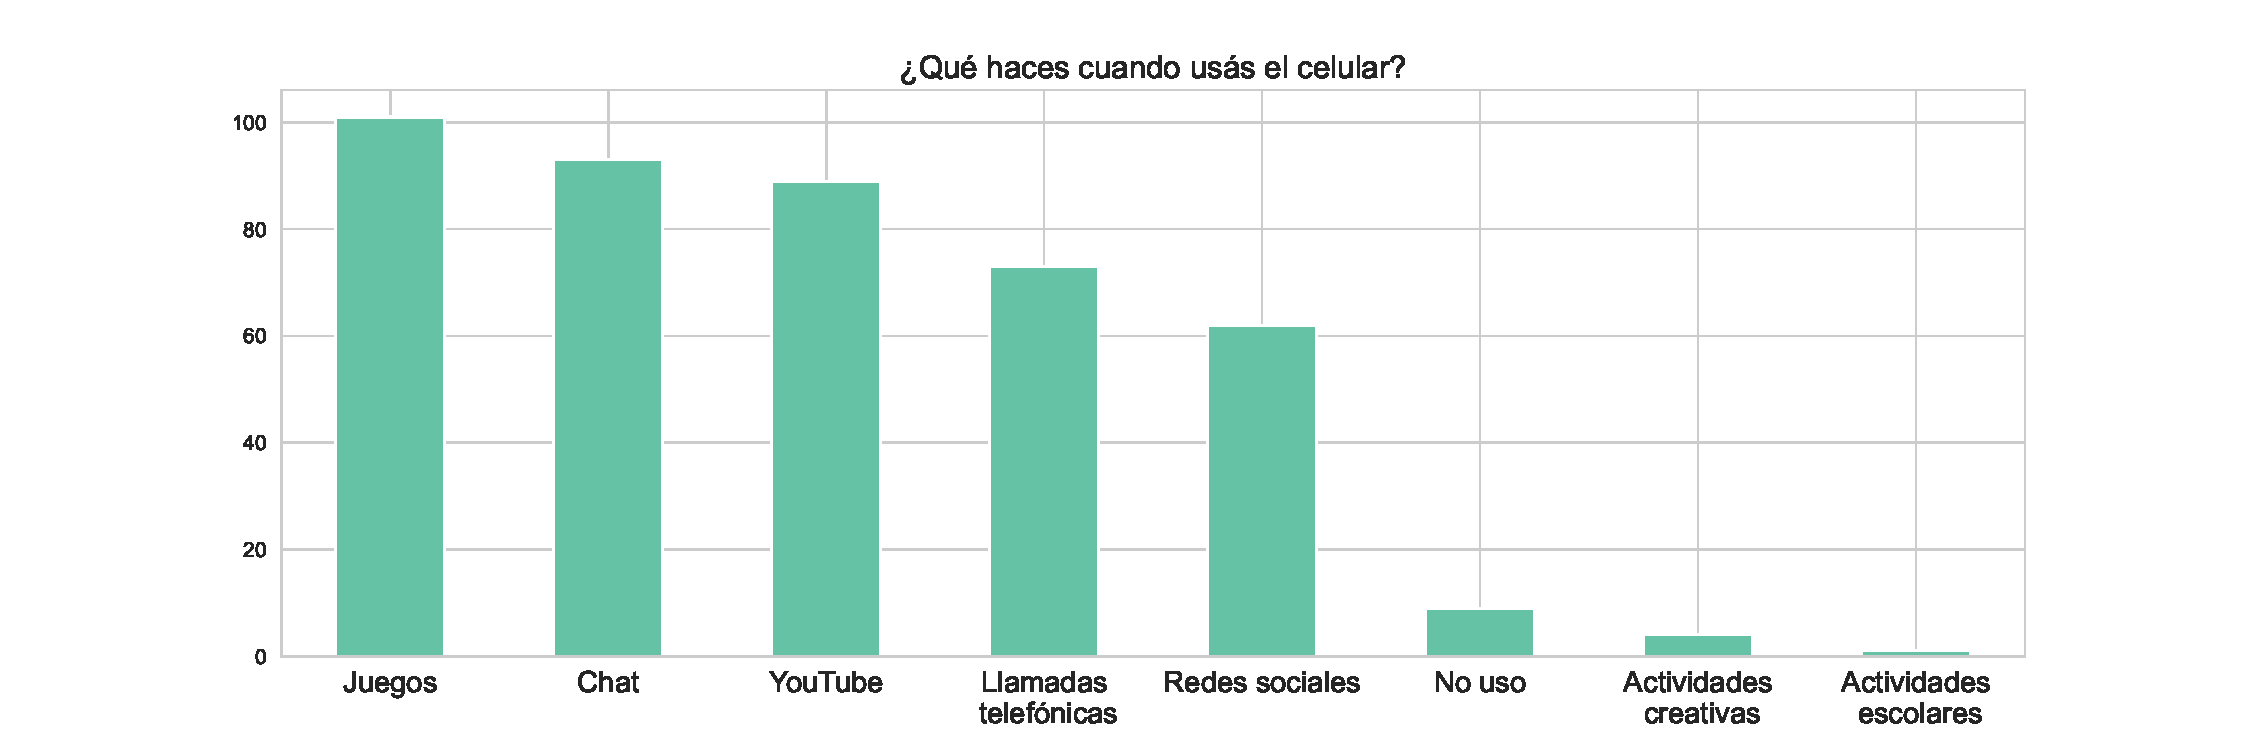
\includegraphics[width=1\textwidth]{images_analisis/7.pdf}
    \caption{Actividades más comunes al utilizar el celular.}
    \label{fig:analisis7}
\end{figure}


Es llamativo que haya aparecido ``\textit{Llamadas telefónicas}'' como una actividad de una importancia considerable, aunque cabe preguntarse si habría que haber pedido que especifiquen si se referían a videollamadas utilizando las aplicaciones anteriormente mencionadas y, en tal caso, la actividad ``\textit{Chat}'' cobraría aún más relevancia.

Dentro de ``\textit{Redes Sociales}'' se incluyen ejemplos como TikTok, Instagram y Facebook, aunque no les pedimos que especifiquen ninguna en particular. Sin embargo, sabemos por la consulta realizada previamente a la confección de la encuesta que realizamos a los referentes pedagógicos de la Fundación Sadosky que trabajan para el Plan Ceibal, que la red social elegida por sobre las otras es en estos momentos TikTok.

Por último, cabe destacar que ``\textit{Actividades creativas}'' no fue una opción propuesta por nosotros en el cuestionario (tanto en esta pregunta como en la relacionada a las actividades realizadas con la computadora), sino que fue agregada por los chicos y chicas al momento de completar la encuesta. Dentro de este grupo, agrupamos respuestas que se referían a la edición de videos y fotos (tal vez para compartir en aplicaciones tales como TikTok o Instagram), escuchar música y escribir historias.

\section{Análisis exploratorio de \textit{misconceptions}}

\subsection{¿Dónde se almacenan los videos de YouTube?}

El primer tema a analizar es el almacenamiento de grandes volúmenes de datos en YouTube. Para esto le preguntamos a los chicos ``\textit{¿Dónde se almacenan los videos que están en YouTube?}'' y les dimos como opciones de respuesta:
\begin{itemize}
    \item En mi celular.
    \item En la nube.
    \item En una computadora.
    \item En muchas computadoras (tantas que podríamos llenar una casa).
    \item En muchísimas computadoras (tantas que podríamos llenar una cancha de fútbol)
    \item No sé.
\end{itemize}

Podemos ver en la Fig. \ref{fig:analisis8} un resultado inicial donde se muestra que la mayoría de ellos respondieron ``\textit{En la nube}''. 

\begin{figure}[h]
    \centering
    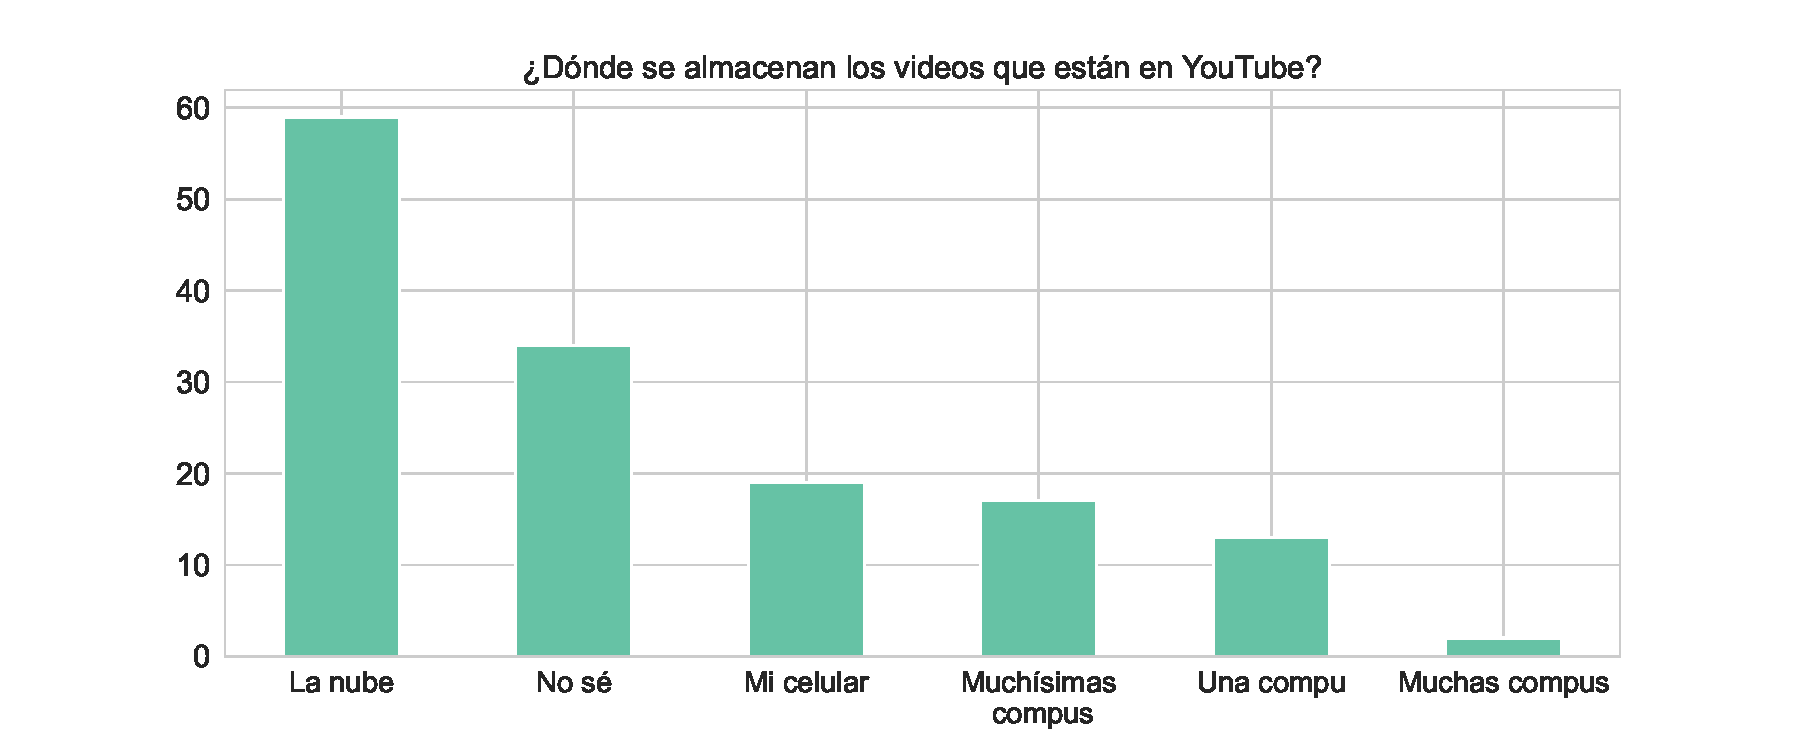
\includegraphics[width=1\textwidth]{images_analisis/8.pdf}
    \caption{Lugar en donde se almacenan los videos que están en YouTube.}
    \label{fig:analisis8}
\end{figure}

Esto es interesante porque el concepto de ``Nube'' es actualmente muy mencionado y por lo tanto está en el léxico de los chicos, a quienes seguramente Google les habrá ofrecido más de una vez ``\textit{más espacio de almacenamiento en la nube}'' (por nombrar un ejemplo). Sin embargo, cabe preguntarse si hay \textit{misconceptions} respecto de este tema puntual: ¿piensan a la nube como algo etéreo? ¿Qué cantidad de información ``entra'' en la nube? ¿Cómo funciona? Este es sin duda un tema interesante para seguir investigando a futuro.

En el siguiente lugar nos encontramos con la respuesta ``\textit{No sé}''. Esto deja en evidencia que este es un tema sobre el cual no se han preguntado mucho, incluso siendo que mirar videos en YouTube es la tercera actividad más elegida (tanto en la computadora como en el celular).

Luego, nos encontramos con una cantidad similar de respuestas con las opciones de ``\textit{En mi celular}'' y en ``\textit{Muchísimas computadoras (tantas que podríamos llenar una cancha de fútbol)}''. En el primer caso, está la \textit{misconception} de que el almacenamiento se da a nivel local, y más aún, que la cantidad de información a almacenar es tal que entraría en un celular. En el segundo caso, nos encontramos con la respuesta que propusimos como la más acertada, en la que queremos transmitir la idea de información distribuida a gran escala.

Por último, están quienes opinaron que la información se guarda en una sola computadora, con la idea de almacenamiento no distribuido, pero tal vez con más capacidad que un celular, y en ``\textit{En muchas computadoras (tantas que podríamos llenar una casa)}'', donde quisimos transmitir una noción de almacenamiento distribuido pero a una escala menor que en la opción de ``Muchísimas computadoras'' (tal vez incluso llevarlos a pensar en que las muchas computadoras podrían encontrarse en una oficina de YouTube o Google, pero todas en un mismo lugar físico).

En la Fig. \ref{fig:analisis9} podemos ver que la cantidad de alumnos con alguna \textit{misconception} en esta pregunta es casi el doble que la de alumnos sin \textit{misconception} (es decir, los niños y niñas que respondieron tanto la respuesta ``correcta'' como ``No sé'').

\begin{figure}[h]
    \centering
    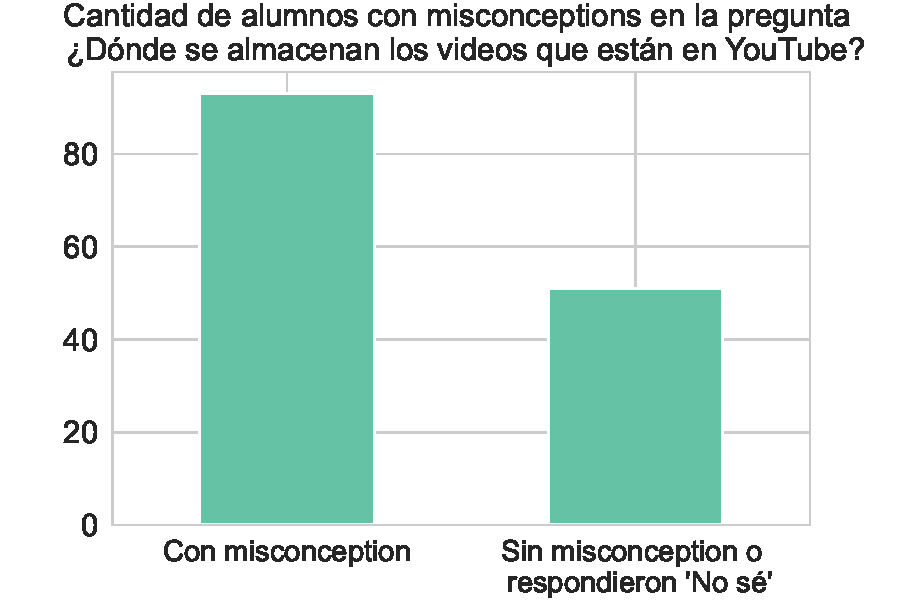
\includegraphics[width=0.6\textwidth]{images_analisis/9.pdf}
    \caption{Alumnos con \textit{misconception} vs sin \textit{misconception} en la pregunta sobre almacenamiento de videos en YouTube.}
    \label{fig:analisis9}
\end{figure}

\newpage

\subsection{¿De qué manera se comparte una foto por WhatsApp?}

La siguiente \textit{misconception} que queremos analizar es cómo es el mecanismo para compartir un archivo por WhatsApp.

En particular, vamos a profundizar en si, al compartir una imagen por este medio, se genera una copia que es la que se envía, o bien se comparte ``por referencia'', es decir, el archivo compartido no le queda en forma de copia a la otra persona, sino que está almacenado en algún servidor o dispositivo de almacenamiento y la persona a la que le fue compartido el archivo puede acceder a él de manera remota.  Más aún: queremos ver si está la noción de que, en este caso, hay un único archivo y que cuando, por ejemplo, éste se modifica, se modifica para todos los que lo ven, y cuando se elimina, se elimina para todos. 

En esta temática, nos pareció que preguntar directamente si una foto se comparte en WhatsApp por copia o referencia iba a generar confusión en los chicos, ya que estos conceptos tal vez no eran conocidos por ellos en estos términos.
De esta forma, pensamos que la mejor estrategia era elaborar un camino de preguntas que de cierto modo pudiera ponerlos en contexto dentro del tema sobre el cual nos interesaba indagar:

\begin{enumerate}
    \item ¿Quién tiene acceso a los archivos que tengo guardados en mi celular?
    \item Cuando comparto por WhatsApp un archivo que tenía guardado, ¿qué sucede? ¿Quién tiene el archivo enviado? ¿De qué manera accede la otra persona al mismo?
    \item ¿Qué pasa si ya no quiero compartir ese archivo? ¿Es posible? ¿Puedo perder la propiedad de un archivo que compartí por WhatsApp?
\end{enumerate}

\newpage

Para esto, la primera pregunta que les hicimos fue ``\textit{¿Quién tiene acceso a las fotos que tengo guardadas en mi celular?}''. En la Fig. \ref{fig:analisis11} podemos ver que la mayoría respondió que solo el dueño o la dueña del celular tiene acceso a las fotos guardadas en el dispositivo. De esta forma, como vemos en la Fig. \ref{fig:analisis10}, es mayor el número de alumnos sin \textit{misconception}.

\begin{figure}[h]
    \centering
    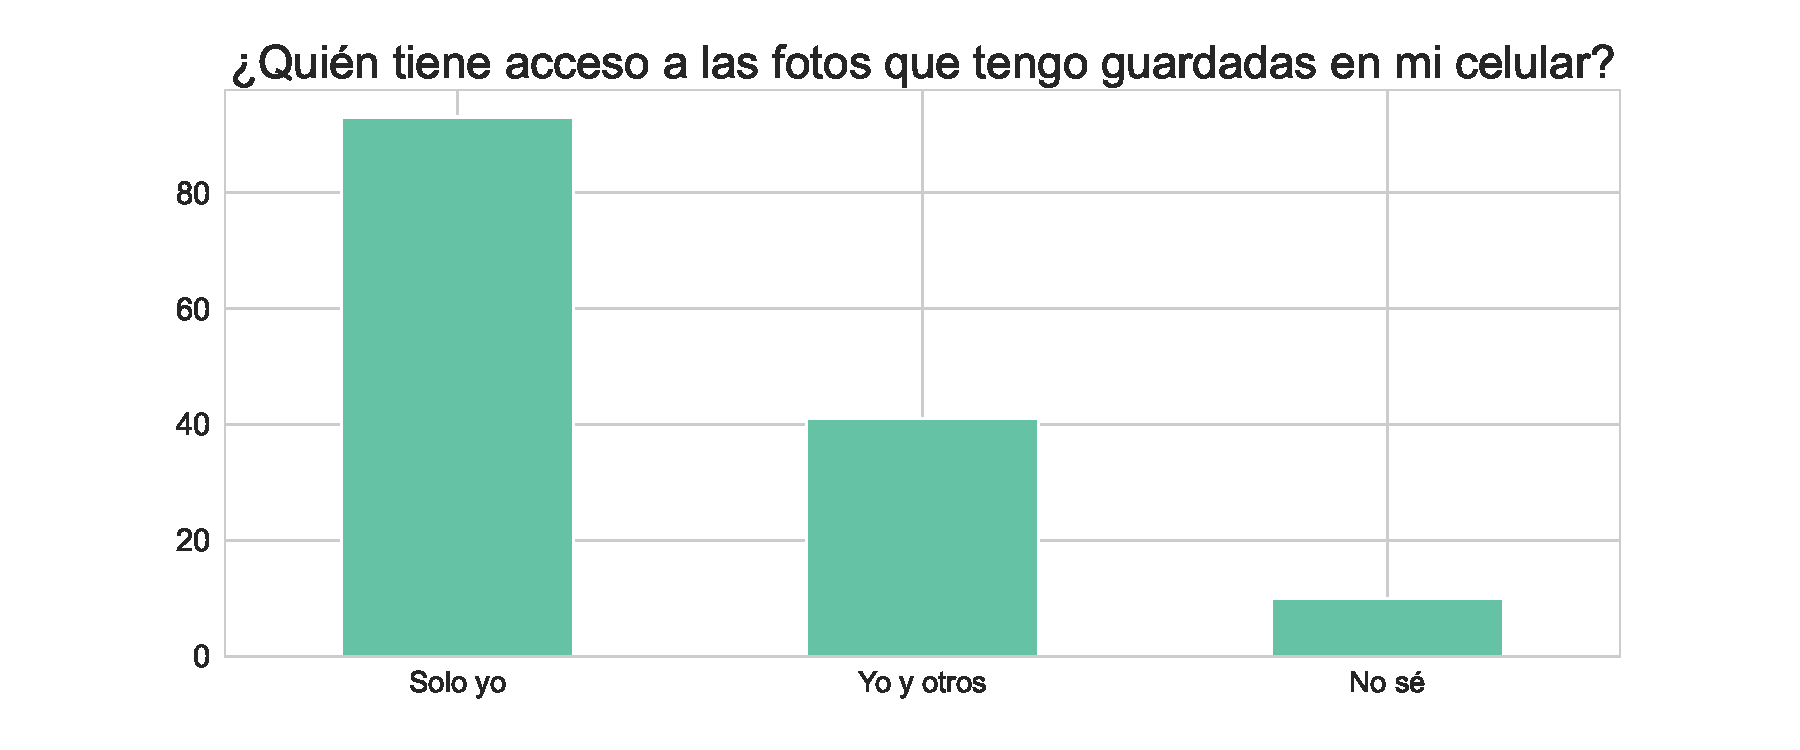
\includegraphics[width=0.8\textwidth]{images_analisis/11.pdf} 
    \caption{¿Quién tiene acceso a las fotos que tengo guardadas en mi celular?}
    \label{fig:analisis11}	
\end{figure}

\begin{figure}[h]
    \centering
    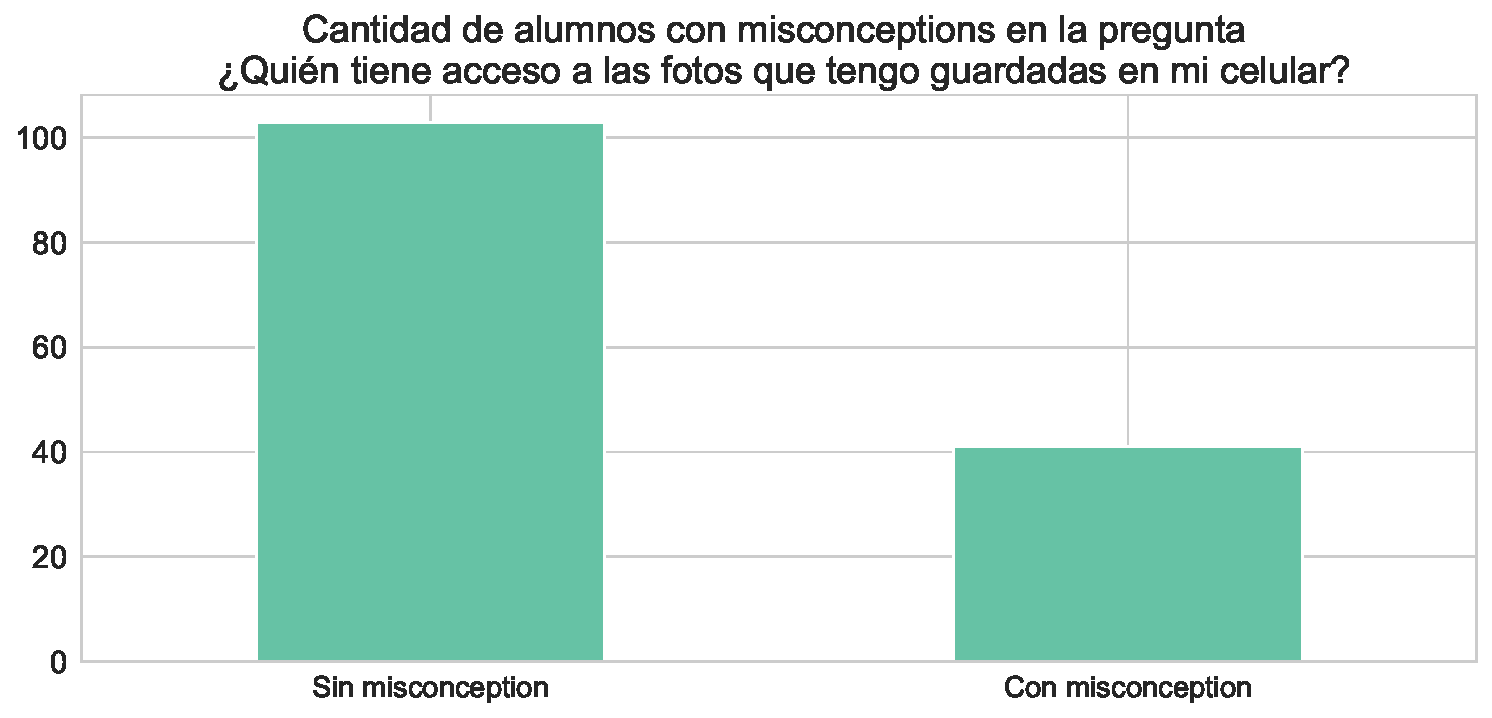
\includegraphics[width=0.8\textwidth]{images_analisis/10.pdf}
    \caption{Alumnos con \textit{misconception} vs sin \textit{misconception} en la pregunta sobre el acceso a fotos en un celular.}
    \label{fig:analisis10}
\end{figure}

Analizando ahora la siguiente pregunta, en la Fig. \ref{fig:analisis12} podemos ver que es bastante similar la cantidad de niños y niñas que opinan, por un lado, que cuando se envía una foto, lo que se manda es una copia y, por el otro, que esa foto ``existe en WhatsApp'' pero que la persona a la que se la enviaron no la tiene como copia en su celular. En esta última opción quisimos dar una idea de referencia.

\begin{figure}[h]
    \centering
    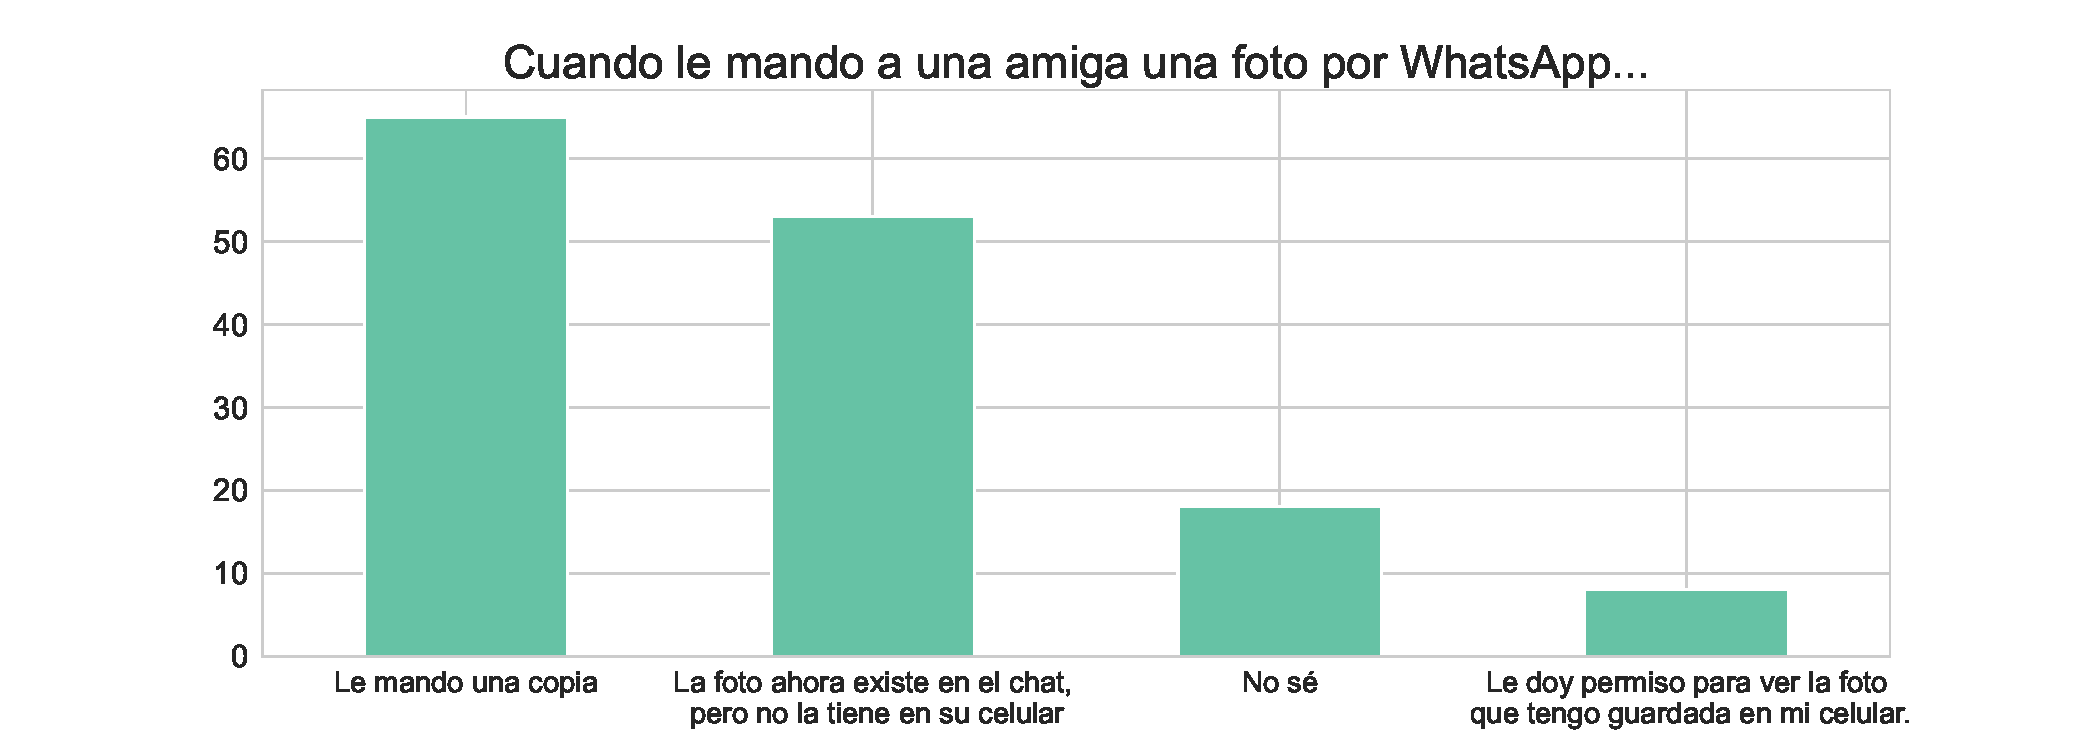
\includegraphics[width=0.9\textwidth]{images_analisis/12.pdf}
    \caption{ ¿Qué pasa cuando le envío a alguien por WhatsApp una foto que tengo en mi celular?}
    \label{fig:analisis12}
\end{figure}

De todas maneras, a pesar de que la respuesta más elegida es la ``correcta'', el número de encuestados y encuestadas con y sin \textit{misconceptions} es parecido. En la Fig. \ref{fig:analisis13} podemos observarlo.

\begin{figure}[h]
    \centering
    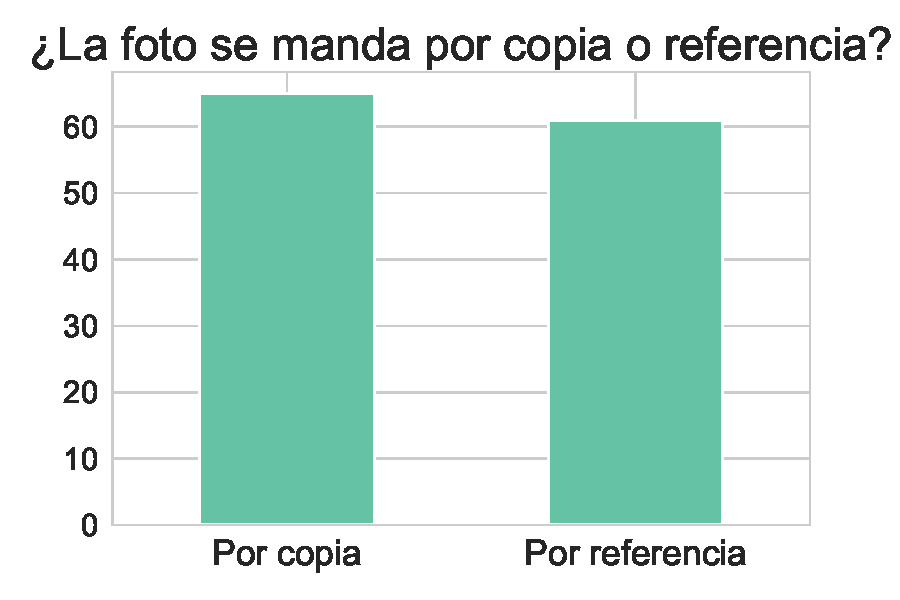
\includegraphics[width=0.4\textwidth]{images_analisis/13.pdf}
    \caption{Niños y niñas que muestran la idea de compartir archivos por copia o por referencia.}
    \label{fig:analisis13}
\end{figure}

\newpage

En la Fig. \ref{fig:analisis15} podemos ver que fueron bastantes los entrevistados que respondieron no saber acerca de este tema. 

\begin{figure}[h]
    \centering
    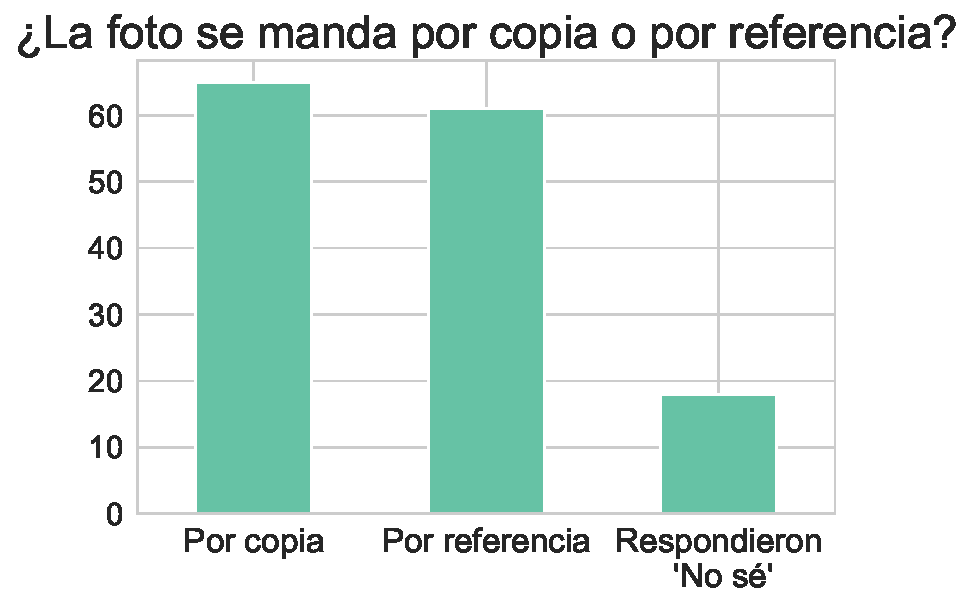
\includegraphics[width=0.4\textwidth]{images_analisis/15.pdf} 
    \caption{Alumnos que respondieron que la foto se manda por copia o referencia, diferenciando los que respondieron "No sé".}
    \label{fig:analisis15}
\end{figure}

\newpage

Sin embargo, considerando que responder “No sé” implica que no se tiene una concepción errónea (ya que justamente, se identifica una falta de conocimiento sobre un tema), podemos considerar a este grupo como dentro de los que no tienen \textit{misconceptions}. De esta forma, la distribución queda como vemos en la Fig. \ref{fig:analisis16}.

\begin{figure}[h]
    \centering
    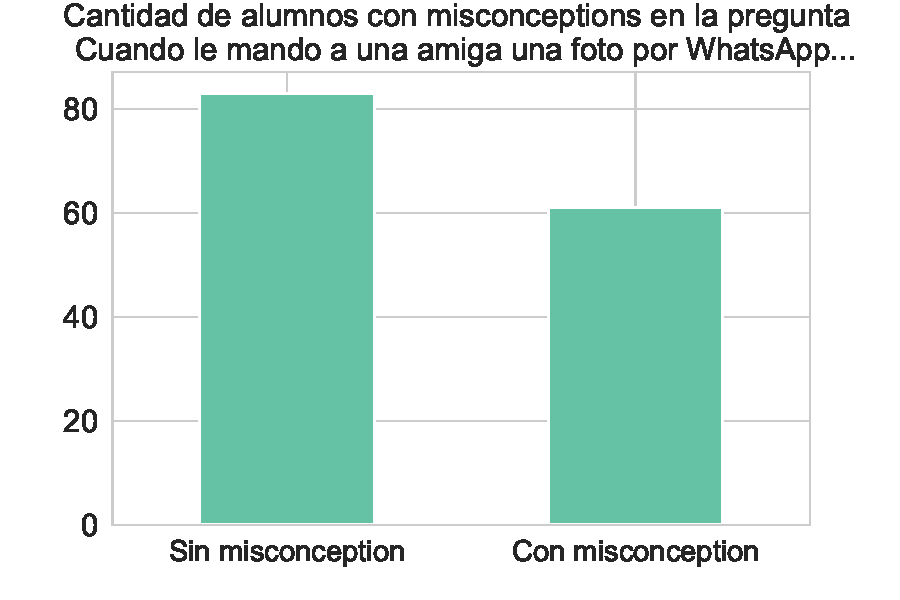
\includegraphics[width=0.5\textwidth]{images_analisis/16.pdf}
    \caption{Cantidad de alumnos con y sin \textit{misconceptions} en la pregunta sobre el envío de una foto por WhatsApp.}
    \label{fig:analisis16}
\end{figure}

Por último, como habíamos mencionado anteriormente en el punto 3, les preguntamos qué pueden hacer si quieren que la persona a la que le compartieron la foto no pueda acceder más a ella. En la Fig. \ref{fig:analisis17} podemos observar las respuestas de los chicos.

\begin{figure}[h]
    \centering
    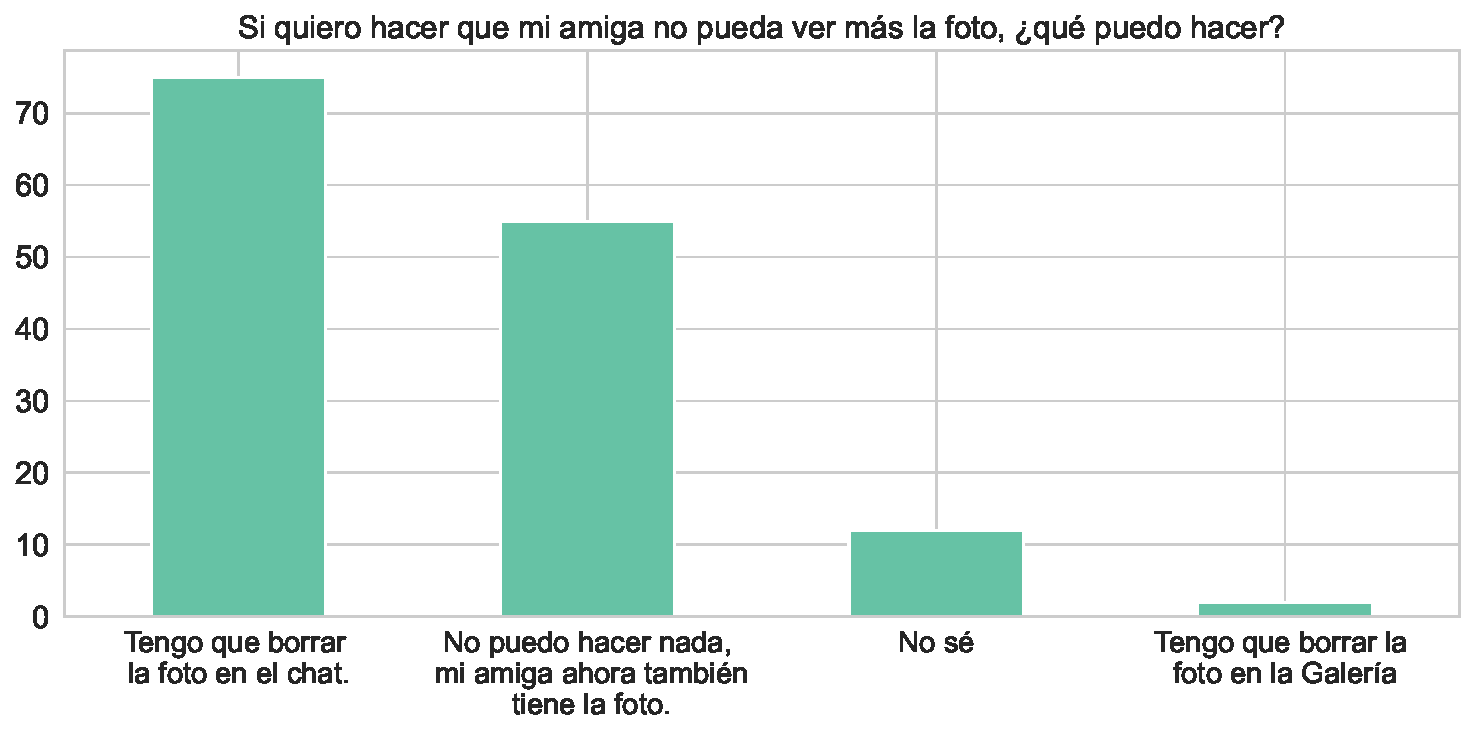
\includegraphics[width=0.95\textwidth]{images_analisis/17.pdf}
    \caption{¿Qué pasa si le compartí a alguien una foto y quiero quitarle el acceso a la misma?}
    \label{fig:analisis17}
\end{figure}

Con esta pregunta, intentamos relacionar los conceptos vistos anteriormente y dilucidar si la idea de copia y referencia estaba clara.

Al analizar los datos, nos encontramos con una sorpresa: si bien en las dos preguntas anteriores, la mayor parte de los niños y niñas encuestadas había contestado correctamente dando a conocer que los archivos se envían como una copia cuando se comparten por WhatsApp, en esta pregunta mostraron tener una \textit{misconception}, tal como se puede ver en la Fig. \ref{fig:analisis18}.

\begin{figure}[h]
    \centering
    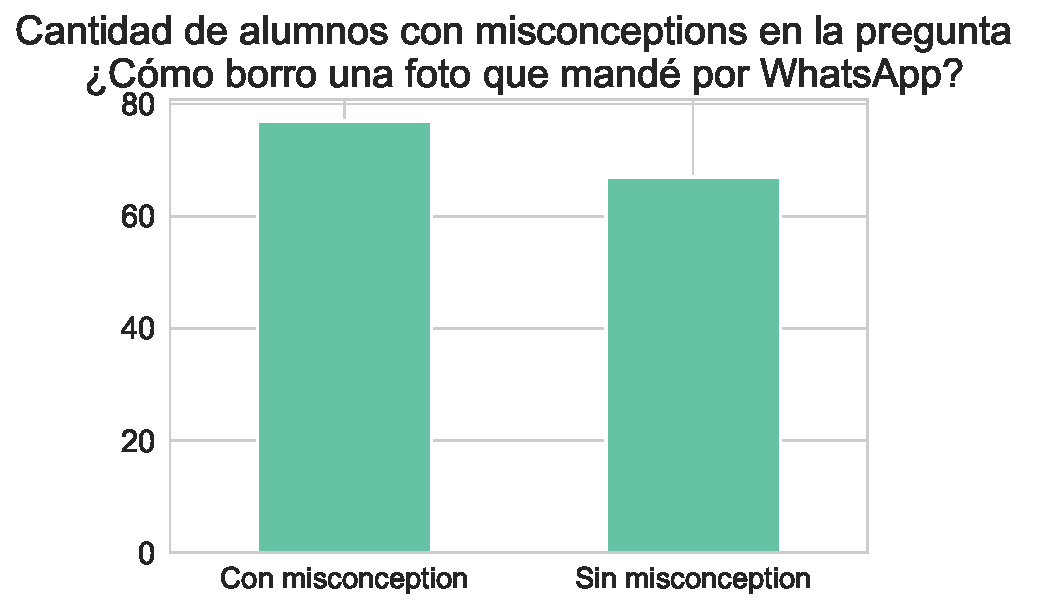
\includegraphics[width=0.5\textwidth]{images_analisis/18.pdf}
    \caption{Cantidad de alumnos con y sin \textit{misconceptions} en la pregunta sobre qué pasa al borrar una foto de un chat.}
    \label{fig:analisis18}
\end{figure}

La opción más elegida fue que \textbf{para dejar de compartir esa foto bastaría con borrarla en el chat de WhatsApp}. Esta respuesta da una idea de que hay una referencia de la foto existente en el servidor de WhatsApp y que al eliminar el mensaje con el archivo en el chat, es suficiente para quitarle el acceso a la otra persona a los datos previamente compartidos.

En contraste, la opción ``No puedo hacer nada, mi amiga ahora también tiene la foto y no tengo manera de sacársela'' intentaba reflejar la idea de que el archivo es compartido mediante una copia, y que una vez que ésta es enviada a la otra persona, se pierde la propiedad sobre la misma y no es posible hacer nada al respecto.
 
\subsection{¿Cómo funciona la red de telefonía móvil?}

El siguiente tema que quisimos explorar fue el funcionamiento de la conectividad móvil. En particular, indagamos sobre cómo viajan los mensajes de WhatsApp cuando no hay WiFi. En la Fig. \ref{fig:analisis19} podemos observar las respuestas obtenidas.

\begin{figure}[h]
    \centering
    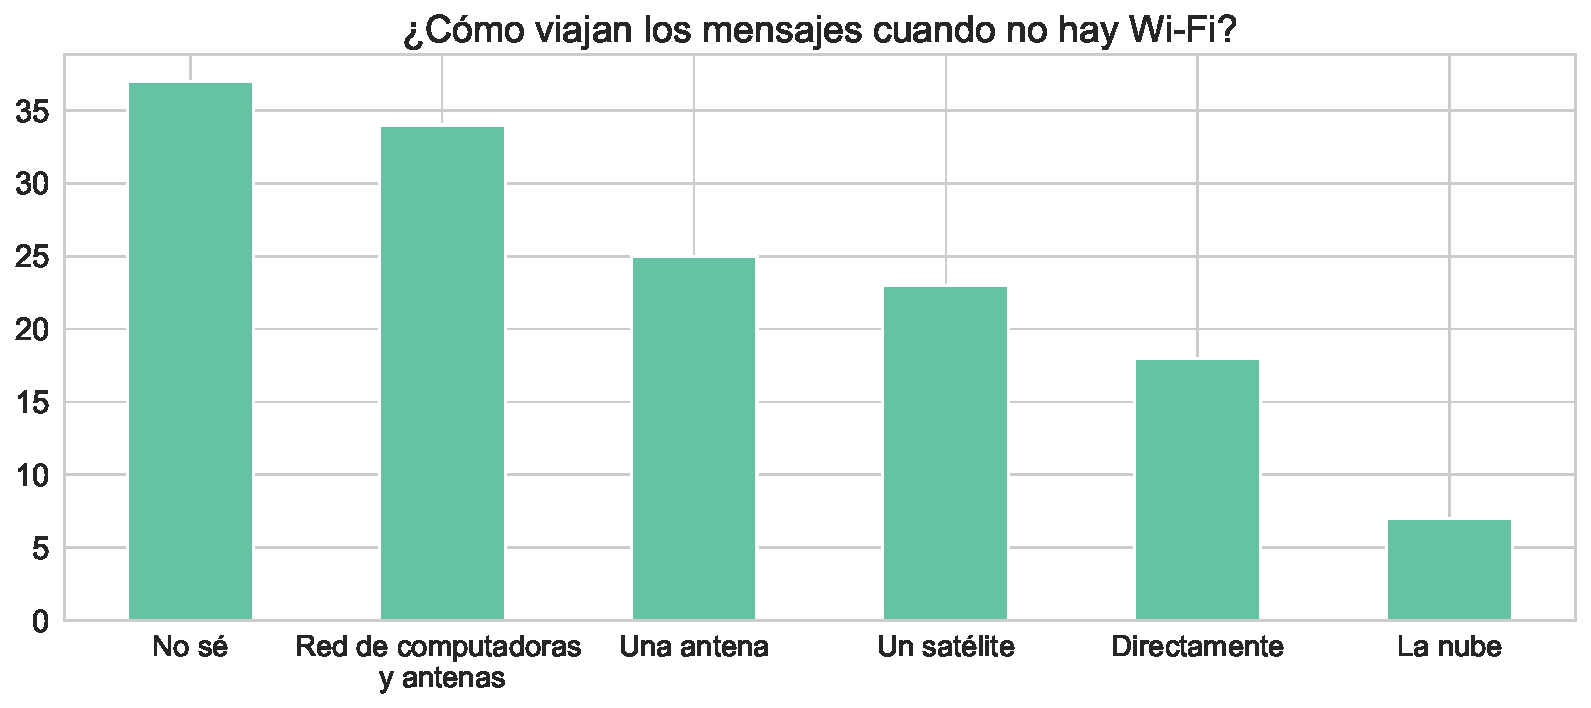
\includegraphics[width=0.9\textwidth]{images_analisis/19.pdf}
    \caption{¿Cómo viajan los mensajes de WhatsApp cuando no hay Wi-Fi?}
    \label{fig:analisis19}
\end{figure}

Es llamativo que en esta pregunta, la opción más elegida fue ``\textit{No sé}''. A pesar de que la gran mayoría de los chicos cuenta con un teléfono celular propio o bien accede a uno que le prestan, vemos que no han llegado a conclusiones respecto a cómo funciona la tecnología de fondo.

De todas formas, una cantidad similar de niños y niñas respondieron a su vez correctamente al elegir la respuesta en la que se proponía que los mensajes viajan a través de una red de antenas y computadoras.
En una proporción semejante aparecen las respuestas en las que se indica que los mensajes viajan a través de una (única) antena, un satélite y ``directamente'' (dando a entender que no existe una infraestructura que intervenga en este proceso).

En la Fig. \ref{fig:analisis20} se muestra un agrupamiento de las respuestas que contienen una \textit{misconception} (en este caso, las que indican que los mensajes viajan a través de la nube, de un satélite, una única antena o directamente) en contraste con la respuesta ``acertada'' (que indicaba que el mensaje viajaba a través de una red de antenas y computadoras) en unión con los que respondieron ``No sé''.

\begin{figure}[h]
    \centering
    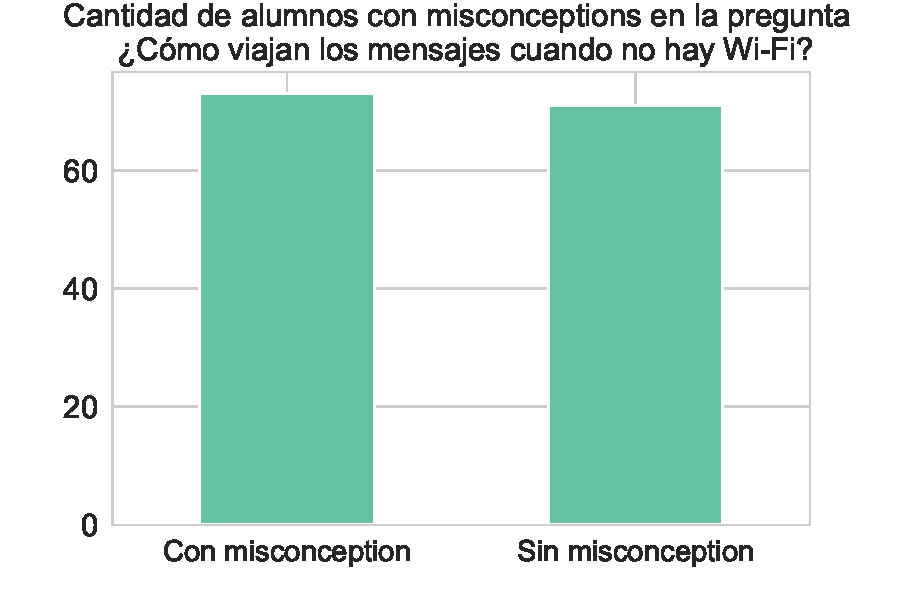
\includegraphics[width=0.6\textwidth]{images_analisis/20.pdf}
    \caption{Cantidad de alumnos con y sin \textit{misconceptions} en la pregunta sobre cómo viajan los mensajes cuando no hay WiFi.}
    \label{fig:analisis20}
\end{figure}

El número de niños y niñas con y sin \textit{misconception} es bastante similar. Veamos ahora si agrupamos las respuestas de otra manera.

\begin{figure}[h]
    \centering
    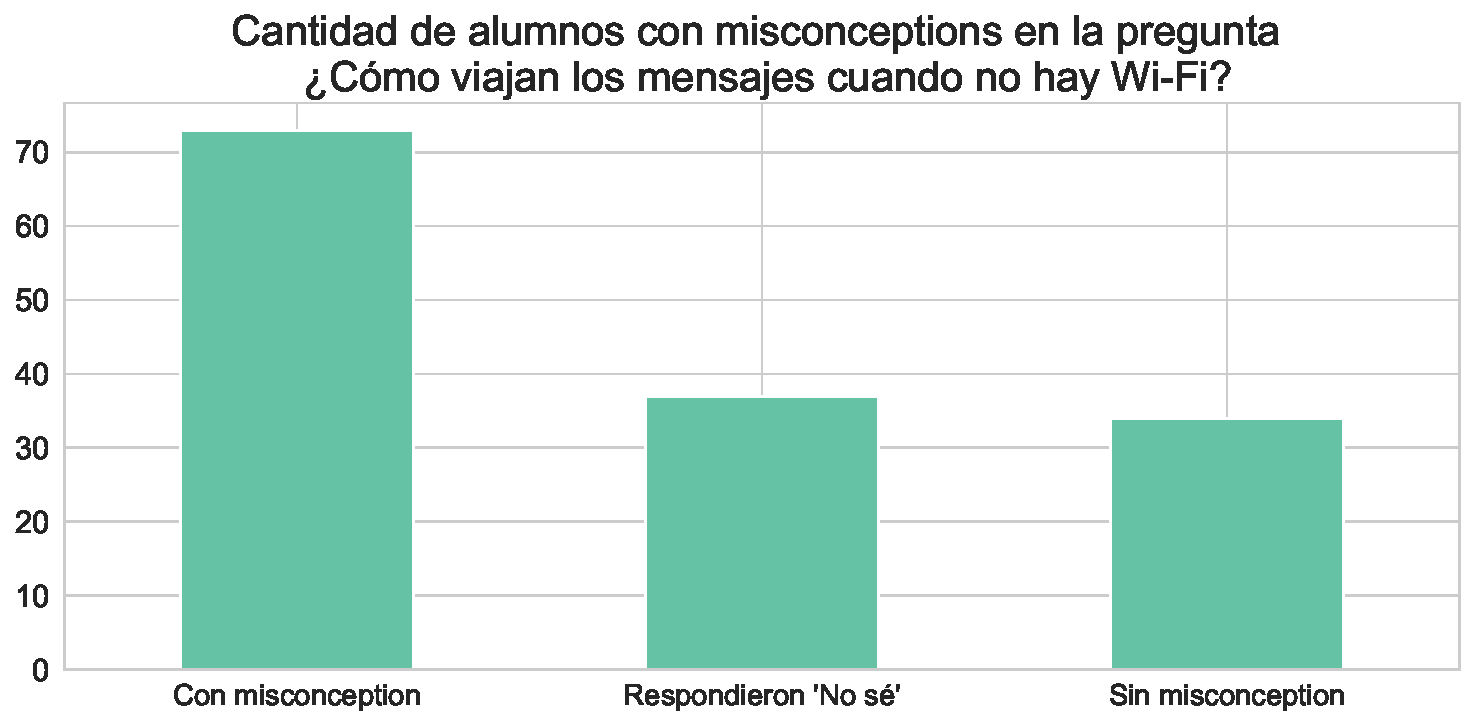
\includegraphics[width=0.7\textwidth]{images_analisis/21.pdf}
    \caption{Alumnos con y sin \textit{misconceptions}, diferenciando a los que respondieron “No sé”.}
    \label{fig:analisis21}
\end{figure}

Si lo analizamos como en la Fig. \ref{fig:analisis21} podemos observar que son más los alumnos que respondieron con \textit{misconception} que los que respondieron correctamente (es decir, sin \textit{misconception}). Más aún: la diferencia es mayor cuando consideramos a los que tienen \textit{misconception} o “no saben”. 

Por último, cabe destacar que la opción de que viajan a través de ``\textit{La nube}'' fue la menos elegida. Y esto es un dato no menor, ya que como habíamos mencionado anteriormente, en la pregunta ``\textit{¿Dónde se almacenan los videos que están en YouTube?}'' la respuesta más elegida fue justamente ``\textit{En la nube}''. Con esta información podemos desentrañar también un poco más cuáles son sus concepciones acerca de ``la nube'': un espacio de almacenamiento ``etéreo'' de datos más que un medio por el cual se envía y recibe información.

\subsection{Gratuidad de las aplicaciones en Internet}


Para conocer las concepciones de los chicos y chicas acerca del por qué de la gratuidad de algunas aplicaciones, les preguntamos ``\textit{¿Por qué hay aplicaciones gratuitas?}'' y, a diferencia de antes, les permitimos a los entrevistados contestar con más de una opción.

\begin{figure}[h]
    \centering
    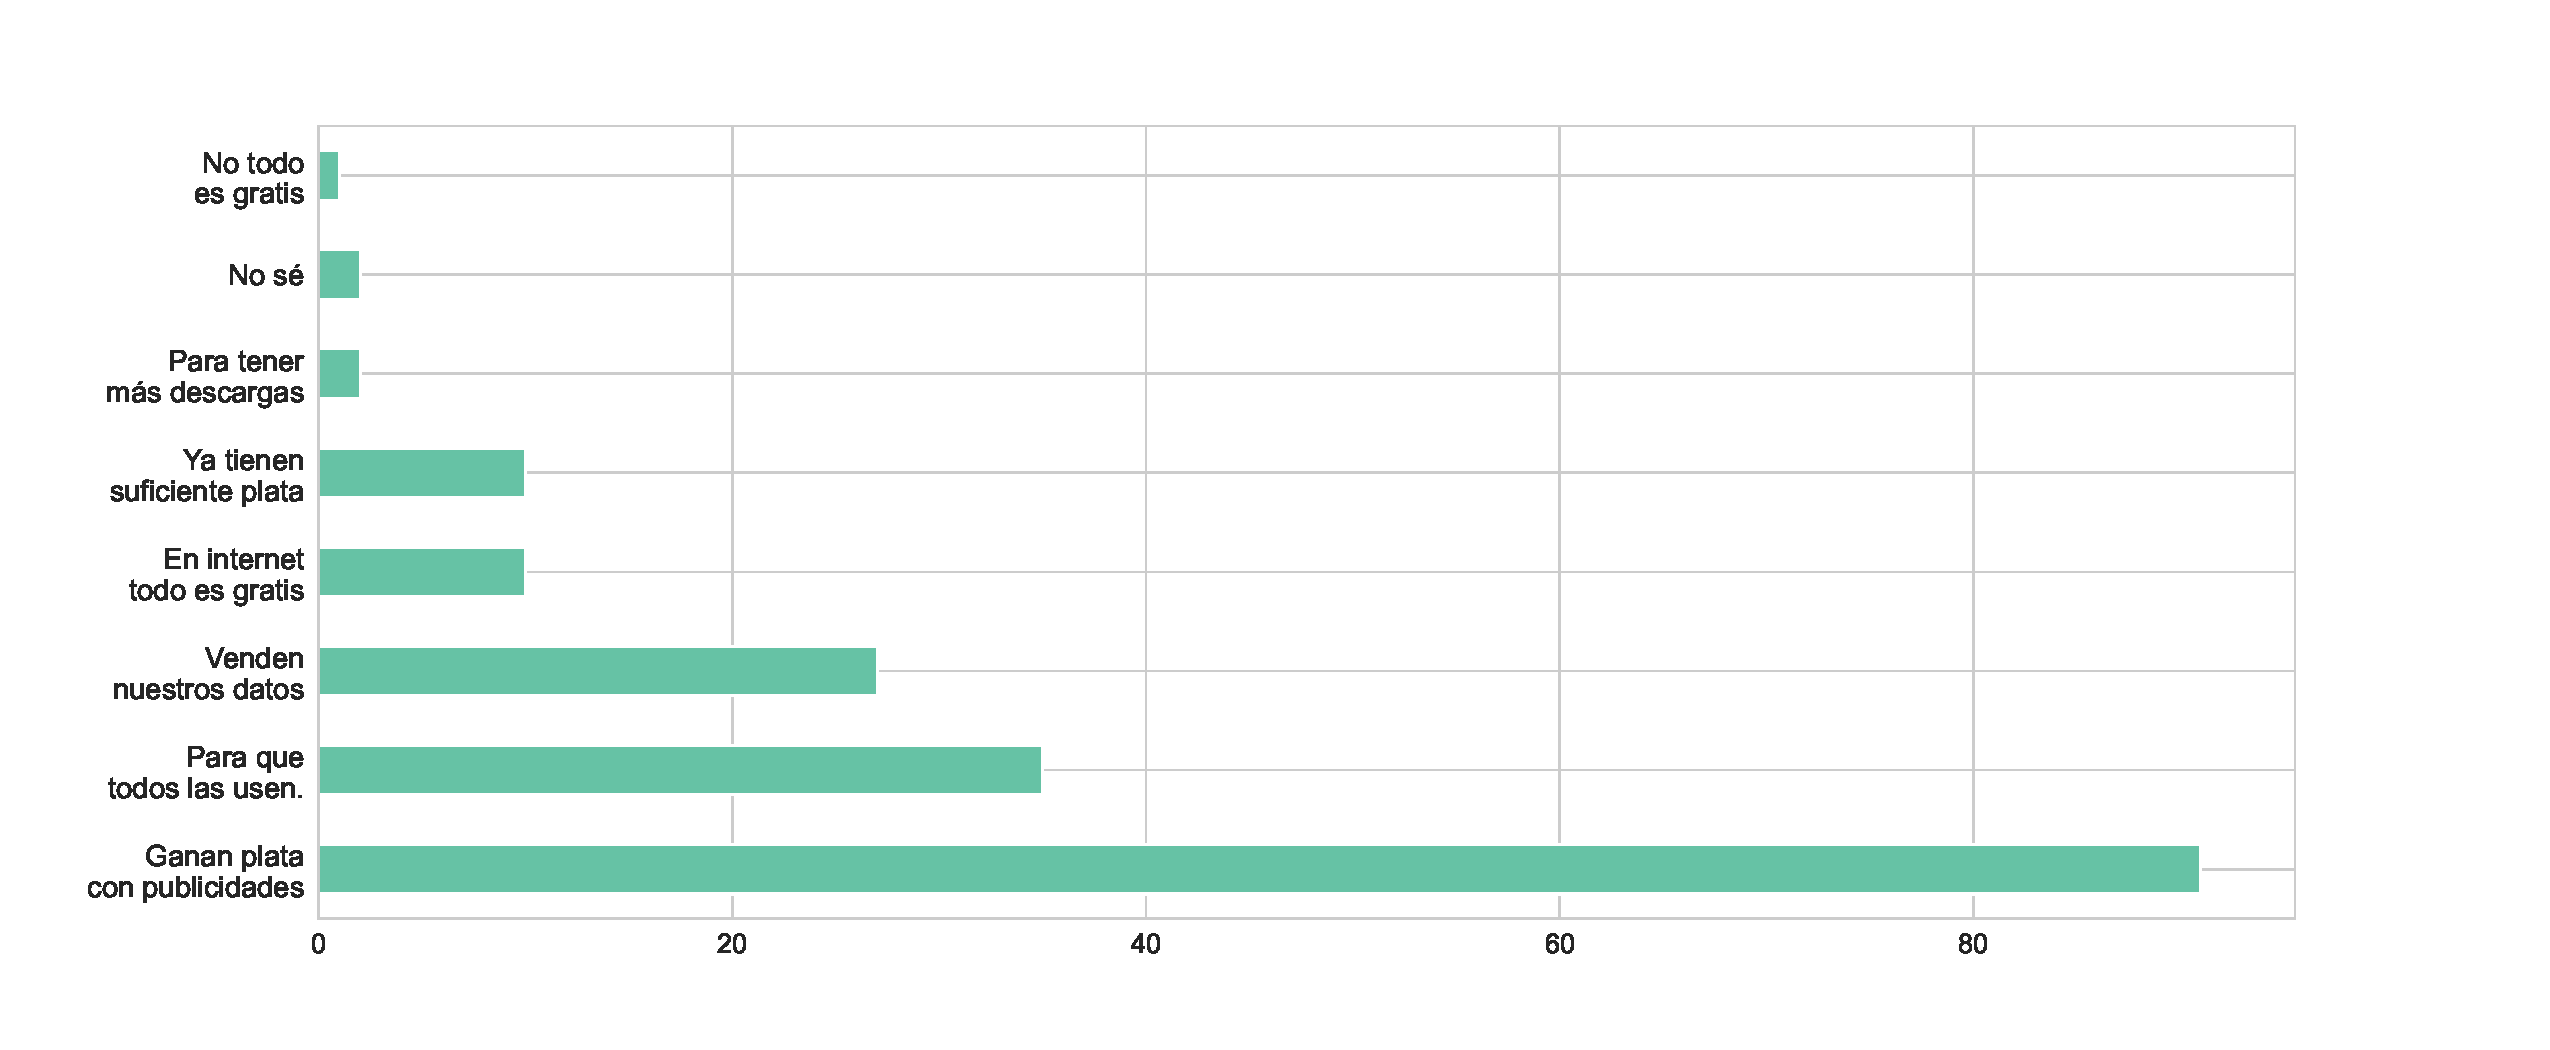
\includegraphics[width=1\textwidth]{images_analisis/22.pdf}
    \caption{Respuestas de la pregunta sobre gratuidad de las aplicaciones, agrupadas por frecuencia de aparición.}
    \label{fig:analisis22}
\end{figure}

En la Fig. \ref{fig:analisis22} mostramos cuáles fueron las opciones más elegidas. La gran mayoría eligió dentro de sus opciones la que propone que la gratuidad de estas es posible gracias al dinero que ganan con las publicidades que nos muestran. Las otras opciones que les habíamos planteado quedaron bastante por detrás en tanto a cantidad de chicos que las eligieron.

Si lo vemos de esta forma, la cantidad de alumnos con y sin \textit{misconception} respecto de este tema es similar, y los que respondieron que no sabían al respecto son realmente muy pocos, como se puede ver en la Fig. \ref{fig:analisis23}.

\begin{figure}[h]
    \centering
    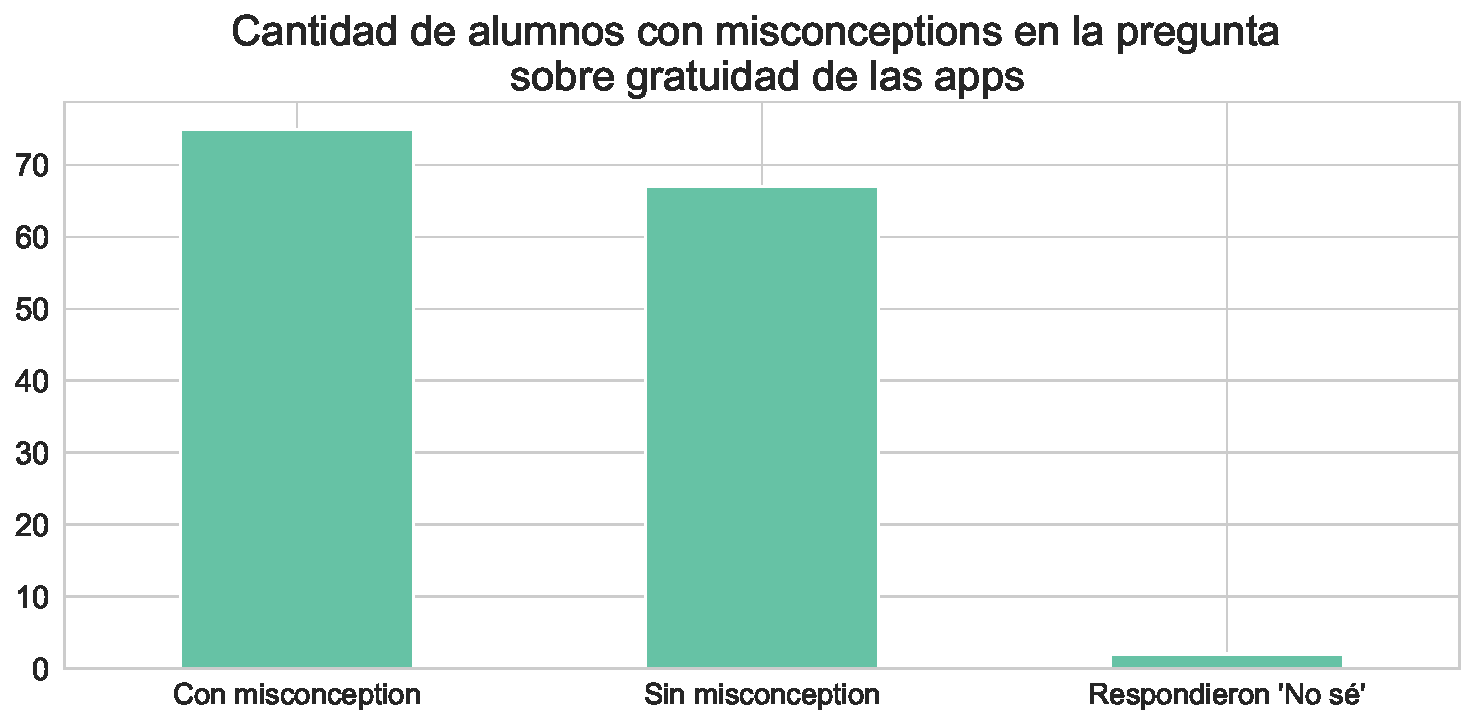
\includegraphics[width=0.75\textwidth]{images_analisis/23.pdf}
    \caption{Cantidad de alumnos con y sin \textit{misconceptions} en la pregunta sobre gratuidad de las aplicaciones en Internet.}
    \label{fig:analisis23}
\end{figure}

\newpage

Sin embargo, dado que en esta pregunta era posible elegir más de una opción, podemos hacer un análisis teniendo en cuenta cuatro grupos: 

\begin{enumerate}
\item Los que respondieron sin \textit{misconception}.
\item Los que respondieron con una \textit{misconception} parcial, es decir, eligieron la respuesta “correcta” junto a otras respuestas con \textit{misconception} (por ejemplo, opinando que las aplicaciones son gratuitas porque ``\textit{ya tienen suficiente dinero y no necesitan más}'' y porque ``\textit{obtienen dinero a través de las publicidades que nos muestran}'').
\item Los que eligieron únicamente respuestas con \textit{misconceptions}.
\item Los que respondieron “No sé”.
\end{enumerate}

\begin{figure}[h]
    \centering
    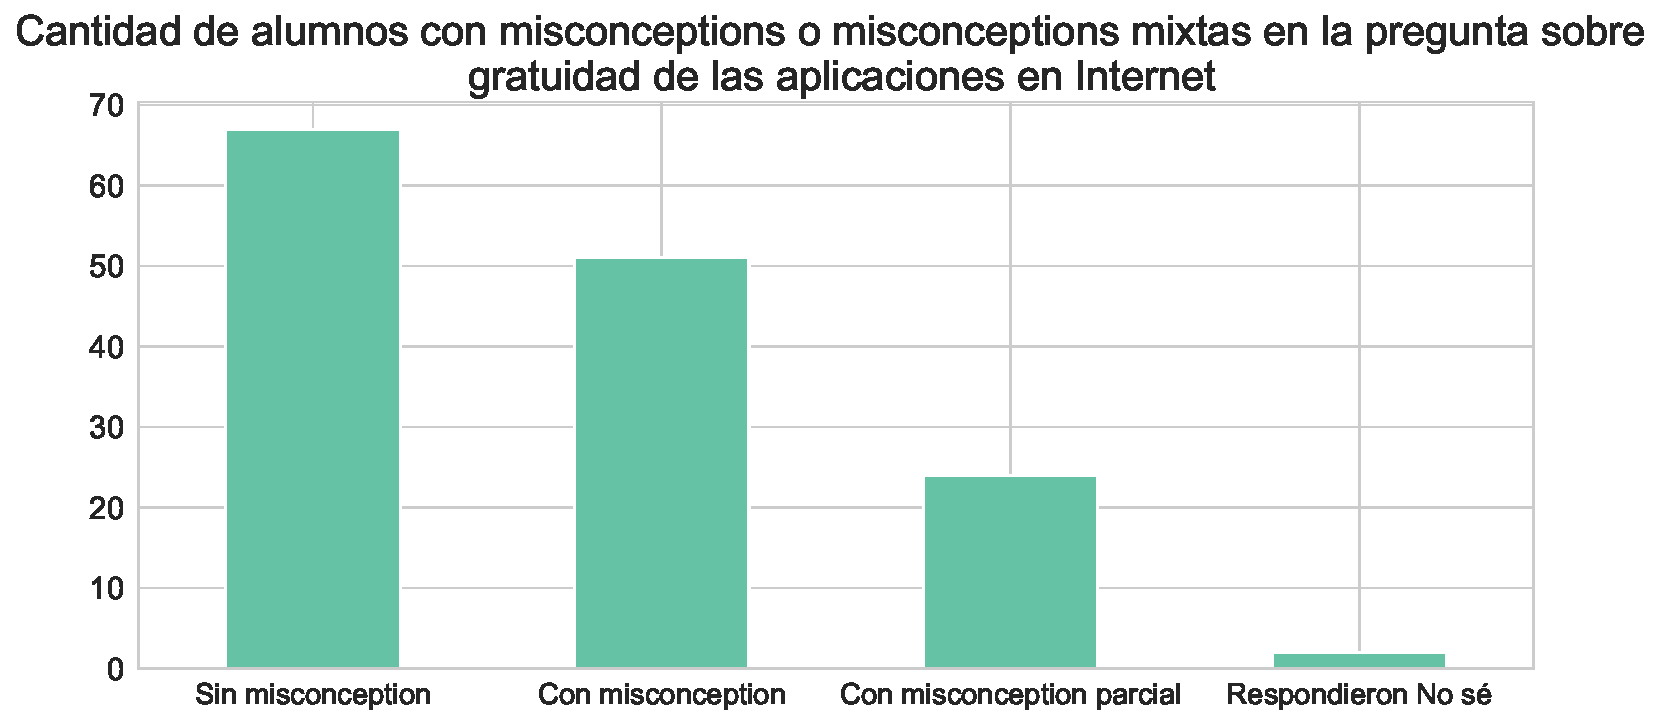
\includegraphics[width=0.75\textwidth]{images_analisis/24.pdf}
    \caption{Cantidad de alumnos con \textit{misconceptions}, sin \textit{misconceptions} y con \textit{misconceptions} parciales en la pregunta sobre gratuidad de las aplicaciones en Internet.}
    \label{fig:analisis24}
\end{figure}


Según esta categorización podemos ver en la Fig. \ref{fig:analisis24} que la cantidad de alumnos sin \textit{misconceptions} es mayor a la cantidad de alumnos con \textit{misconceptions}, o con \textit{misconceptions} parciales.

Es interesante mencionar que en esta pregunta habíamos dejado un casillero libre para completar con otras opciones que se les pudiesen ocurrir y que no estuvieran disponibles. De esta forma, algunos completaron que las aplicaciones son gratis para poder conseguir así ``más descargas en el Play Store''. Según esta respuesta, las aplicaciones ganan más dinero cuantas más descargas consiguen.

La otra respuesta proporcionada por los chicos y chicas fue que ``\textit{No todo es gratis}'' en Internet, dando a entender que también hay aplicaciones que no son gratuitas.

\section{Relación entre las \textit{misconceptions}}

Analicemos ahora si es posible encontrar una relación entre las \textit{misconceptions} que hay en los distintos temas.

Para mayor claridad, nombraremos a las preguntas realizadas para evaluar la presencia o no de \textit{misconceptions} de la siguiente manera:

\begin{table}[h]
\centering
\resizebox{\textwidth}{!}{%
\begin{tabular}{|l|l|}
\hline
¿Dónde se almacenan los videos que están en YouTube? & Pregunta  YouTube     \\ \hline
¿Quién tiene acceso a las fotos que tengo guardadas en mi celular?           & Pregunta Acceso Fotos     \\ \hline
Cuando le mando a una amiga una foto por WhatsApp…   & Pregunta Mandar Fotos \\ \hline
Si quiero hacer que mi amiga no pueda ver más la foto, ¿qué puedo hacer?     & Pregunta Borrar Fotos     \\ \hline
Sofi está en la calle sin WiFi y le quiere mandar un mensaje de WhatsApp.... & Pregunta Mensaje sin WiFi \\ \hline
Muchas de las aplicaciones que conocemos se pueden usar gratuitamente...     & Pregunta Gratuidad Apps   \\ \hline
\end{tabular}%
}
\end{table}

En primer lugar,  revisemos cuántas \textit{misconceptions} tiene cada alumno o alumna en general. En la Fig. \ref{fig:analisis25}, podemos observar que la mayoría de los niños y niñas entrevistados tiene al menos 2 \textit{misconceptions}.

\begin{figure}[h]
    \centering
    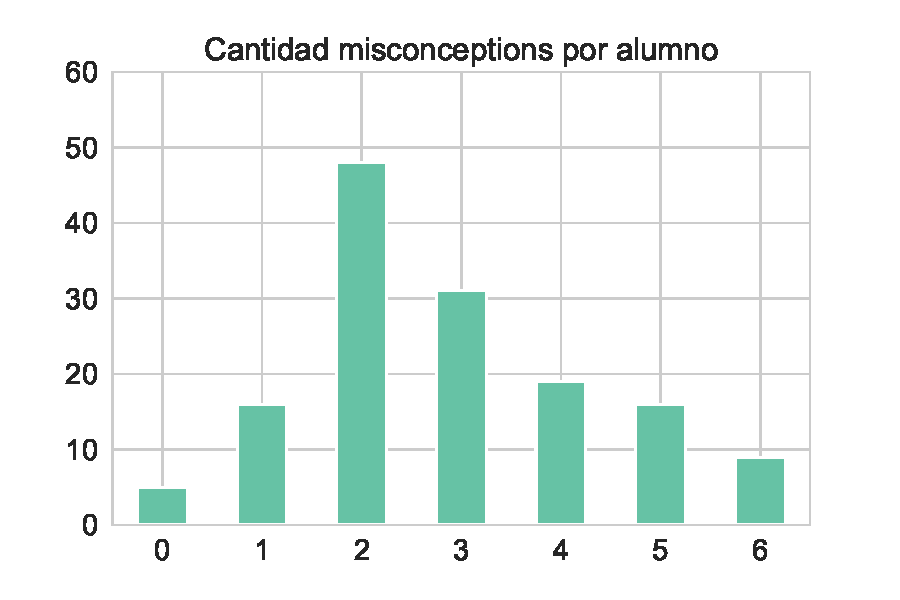
\includegraphics[width=0.55\textwidth]{images_analisis/25.pdf}
    \caption{Cantidad de \textit{misconceptions} por alumno.}
    \label{fig:analisis25}
\end{figure}

Es interesante destacar que tan solo 5 encuestados (es decir, el 3,47\% del total) respondieron a todas las preguntas sin presentar una \textit{misconception}.

Por otro lado, si ordenamos las preguntas en función de cuántos alumnos las respondieron mostrando una \textit{misconception}, podemos ver, como se muestra en la Fig. \ref{fig:analisis26}, que la pregunta ``\textit{¿Dónde se almacenan los videos que están en YouTube?}'' es la que aparece en primer lugar.

\begin{figure}[h]
    \centering
    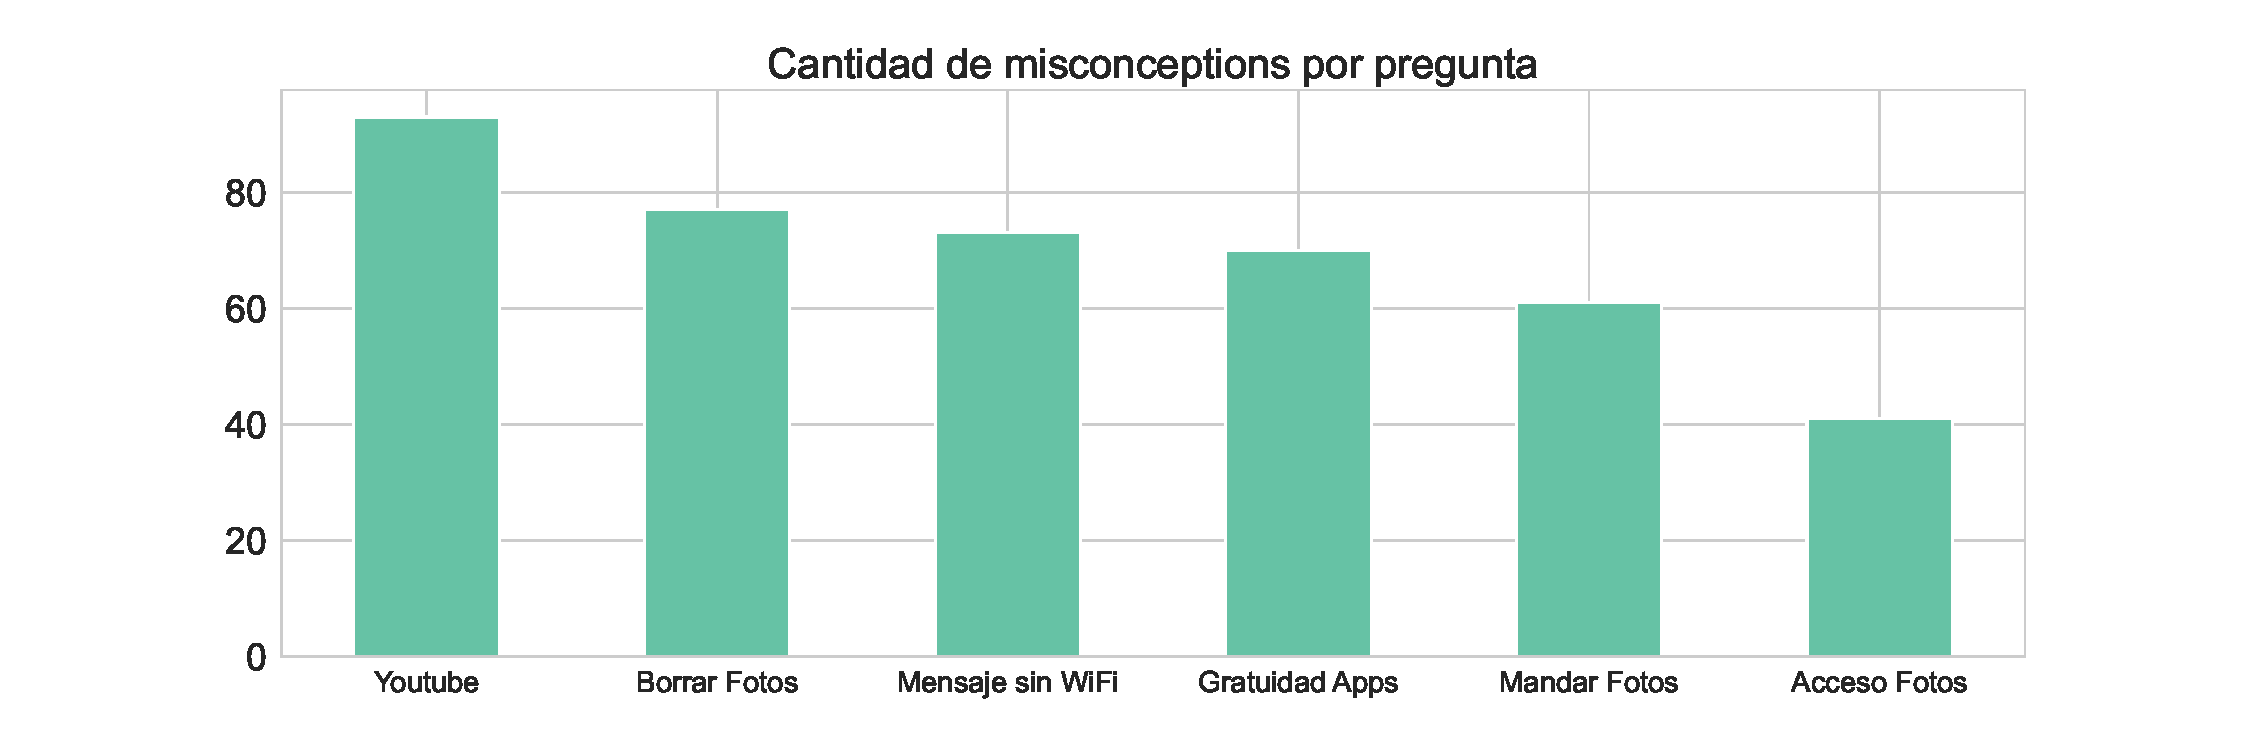
\includegraphics[width=1\textwidth]{images_analisis/26.pdf}
    \caption{\textit{Misconceptions} por pregunta, donde \textit{misconception} parcial no se considera \textit{misconception}.}
    \label{fig:analisis26}  
\end{figure}

\newpage

En segundo lugar, tenemos la pregunta relacionada a si es posible que una persona a la que le compartimos una foto por WhatsApp deje de tener acceso a ésta (``\textit{Si quiero hacer que mi amiga no pueda ver más la foto, ¿qué puedo hacer?}'').

Con casi la misma cantidad de \textit{misconceptions} aparecen la pregunta acerca de cómo viajan los mensajes de WhatsApp cuando no hay WiFi y la pregunta sobre la gratuidad de las aplicaciones en Internet. Sobre esta última cabe destacar que aquí consideramos como \textbf{sin} \textit{misconception} a:

\begin{enumerate}
    \item Los que tenían una \textit{misconception} parcial.
    \item Los que no tenían \textit{misconception}.
    \item Los que respondieron “No sé”.
\end{enumerate}

Si consideramos a los que tenían \textit{misconception} parcial como \textbf{con} \textit{misconception}, entonces como vemos en la Fig. \ref{fig:analisis27}, la distribución cambia y hay más \textit{misconceptions} en esta pregunta que en la de ``\textit{Cómo viajan los mensajes cuando no hay WiFi}''.

\begin{figure}[h]
    \centering
    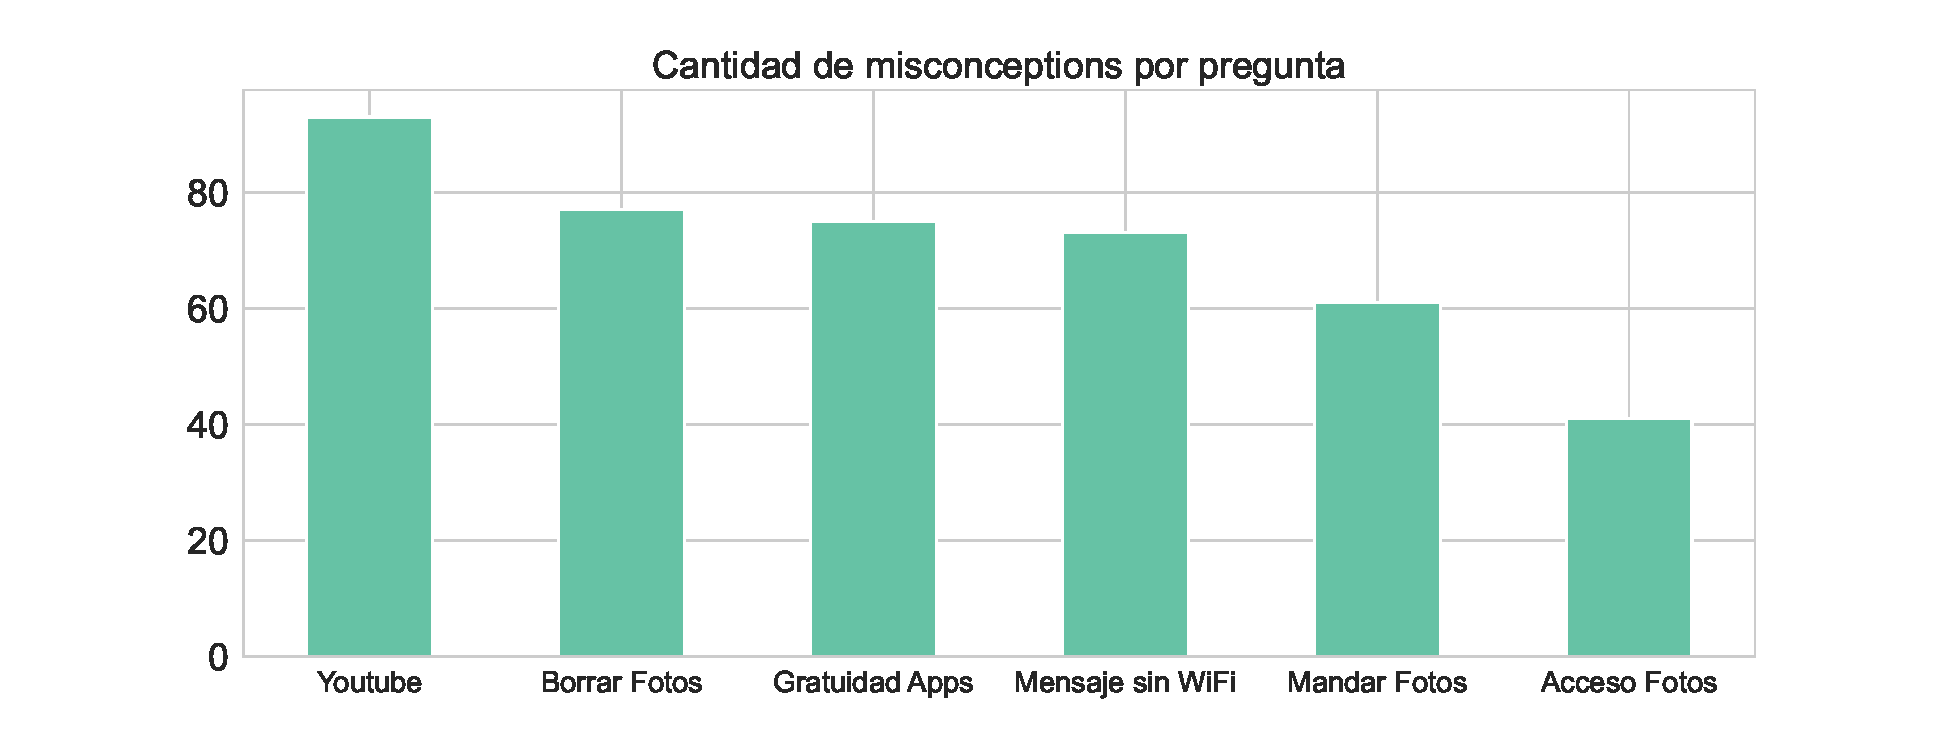
\includegraphics[width=1\textwidth]{images_analisis/27.pdf} 
    \caption{\textit{Misconceptions} por pregunta, donde \textit{misconception} parcial se considera \textit{misconception}.}
    \label{fig:analisis27}
\end{figure}

Por último, analizamos si existe una relación entre las \textit{misconceptions} en las distintas preguntas.

Consideramos para cada pregunta el hecho de si había o no una \textit{misconception} como una variable aleatoria binaria (0 = “no hay \textit{misconception}”, 1 = “hay \textit{misconception}”) y luego medimos la correlación lineal entre ellas usando el método de Pearson. 

Este método devuelve como resultado un valor entre -1 y 1, donde 1 indica una fuerte correlación positiva entre las dos variables (cuando una de las variables es 1 = “hay \textit{misconception}”, la otra también lo es) y -1 muestra una correlación negativa (cuando una de las variables es 1 = “hay \textit{misconception}” la otra es 0 = “no hay \textit{misconception}”). Los valores cercanos a 0 indican que no hay correlación entre las variables.

El \textit{heatmap} que observamos en la Fig. \ref{fig:analisis28} muestra el resultado. 

\begin{figure}[h]
    \centering
    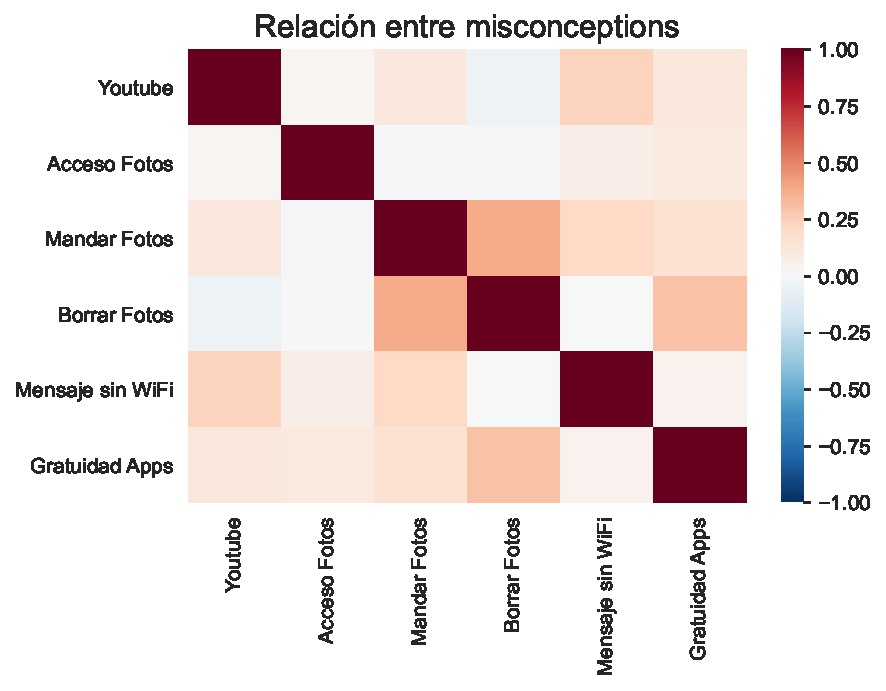
\includegraphics[width=0.7\textwidth]{images_analisis/28.pdf}
    \caption{Relación entre \textit{misconceptions} en las distintas preguntas. }
    \label{fig:analisis28}
\end{figure}

Podemos ver aquí que las preguntas más relacionadas son: ``\textit{Mandar Fotos}'' y ``\textit{Borrar Fotos}''. En ambas buscábamos entender si hay \textit{misconceptions} respecto de si el envío de fotos al utilizar el servicio de mensajería móvil se realiza por copia o referencia, por lo tanto tiene sentido que haya \textit{misconceptions} en ambas preguntas a la vez.

También podemos observar que la pregunta ``\textit{Borrar Fotos}'' se relaciona con ``\textit{Gratuidad Apps}''.

Al mismo tiempo, la pregunta ``\textit{YouTube}'' se encuentra relacionada con ``\textit{Mensajes sin WiFi}''. 

Veamos cómo se relacionan las respuestas de los pares de preguntas, centrándonos en la relación entre las preguntas ``\textit{Mandar Fotos}'' y ``\textit{Borrar Fotos}'' y  ``\textit{YouTube}'' y ``\textit{Mensajes sin WiFi}'' y veamos si este análisis aporta más claridad para entender las relaciones entre las distintas preguntas.

Utilizaremos la siguiente nomenclatura para abreviar las distintas respuestas:

\begin{table}[h]
\centering
\resizebox{\textwidth}{!}{%
\begin{tabular}{|l|l|}
\hline
YouTube - En mi celular                                                               & YouTube - Una compu     \\ \hline
YouTube -  En una computadora                                                         & YouTube - Celular       \\ \hline
YouTube - En la nube                                                                  & YouTube - Nube          \\ \hline
YouTube - En muchas computadoras (tantas que podrían llenar una casa)                 & YouTube - Muchas compus \\ \hline
YouTube - En muchísimas computadoras (tantas que podrían llenar una cancha de fútbol) & YouTube - Muchísimas compus \\ \hline
YouTube - No sé                                                                       & YouTube - No sé         \\ \hline
Mensaje sin WiFI - El mensaje se manda directamente.                                  & Sin WiFi - Directamente \\ \hline
Mensaje sin WiFI - El mensaje se manda a través de la nube.                           & Sin WiFi - Nube         \\ \hline
Mensaje sin WiFI - El mensaje se manda a través de un satélite.                       & Sin WiFi - Satélite     \\ \hline
Mensaje sin WiFI - El mensaje se manda a través de una antena.                        & Sin WiFi - Antena       \\ \hline
Mensaje sin WiFi - El mensaje se manda a través de una red de antenas y computadoras. & Sin WiFi - Red          \\ \hline
Mensaje sin WiFI - No sé                                                              & Sin WiFi - No sé        \\ \hline
Borrar Fotos - Tengo que borrar la foto en el chat.                                   & Borrar - En el chat     \\ \hline
Borrar Fotos - Tengo que borrar la foto en la Galería de fotos de mi celular.         & Borrar - En mi celu     \\ \hline
Borrar Fotos - No puedo hacer nada...                                                 & Borrar - No puedo       \\ \hline
Borrar Fotos - No sé                                                                  & Borrar - No sé          \\ \hline
Mandar Fotos - Le doy permiso para ver la foto que tengo guardada en mi celular.      & Mandar - En mi celu     \\ \hline
Mandar Fotos - Le mando una copia de mi foto                                          & Mandar - copia          \\ \hline
Mandar Fotos - La foto ahora existe en WhatsApp...                                    & Mandar - En WhatsApp    \\ \hline
Mandar Fotos - No sé                                                                  & Mandar - No sé          \\ \hline
\end{tabular}%
}
\end{table}

\newpage

En todos los casos, consideramos como hicimos anteriormente, a cada posible respuesta como una variable aleatoria binaria, donde 0 es “No se eligió dicha respuesta” y 1 es “Se eligió dicha respuesta”. Comprobaremos si hay una correlación lineal entre los pares de preguntas utilizando nuevamente el método de Pearson.

\begin{figure}[h]
    \centering
    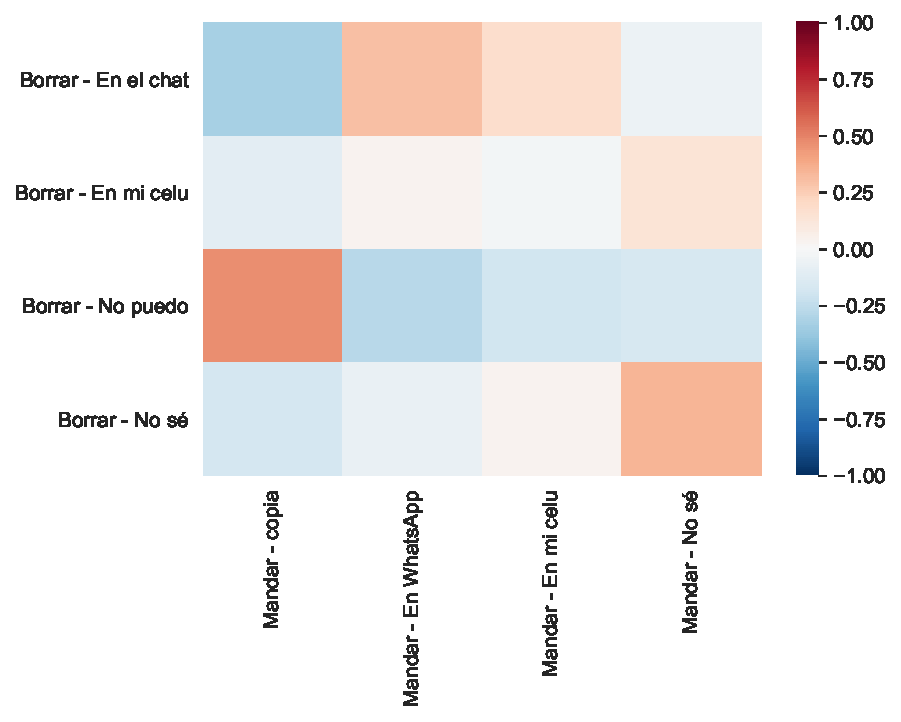
\includegraphics[width=0.7\textwidth]{images_analisis/29.pdf}
    \caption{Relación entre las respuestas a las preguntas “Mandar Fotos” y “Borrar Fotos”.}
    \label{fig:analisis29}
\end{figure}

En la Fig. \ref{fig:analisis29} podemos ver que para las preguntas ``\textit{Mandar Fotos}'' y ``\textit{Borrar Fotos}'' las respuestas que parecieran estar más correlacionadas positivamente (es decir, mayormente los alumnos eligieron estas dos respuestas al responder la encuesta) son:

\begin{itemize}
    \item Borrar- No puedo.
    \item Mandar - copia.
    \item Mandar - No se.
    \item Borrar - No se.
    \item Borrar - En el chat.
    \item Mandar - En WhatsApp.
\end{itemize}

También notamos que hay correlaciones negativas, es decir, mayormente los alumnos no eligieron estas respuestas al mismo tiempo, entre las respuestas:

\begin{itemize}
    \item Borrar - En el chat.
    \item Mandar - copia.
    \item Borrar- No puedo.
    \item Mandar - En WhatsApp.
\end{itemize}

En el caso de las preguntas ``\textit{YouTube}'' y ``\textit{Mensajes sin WiFi}'', es posible observar en la Fig. \ref{fig:analisis30} que las respuestas más correlacionadas positivamente son:

\begin{itemize}
    \item YouTube - Una compu
    \item Sin WiFi - Directamente.
    \item YouTube - Celular.
    \item WiFi - Directamente.
\end{itemize}

\begin{figure}[h]
    \centering
    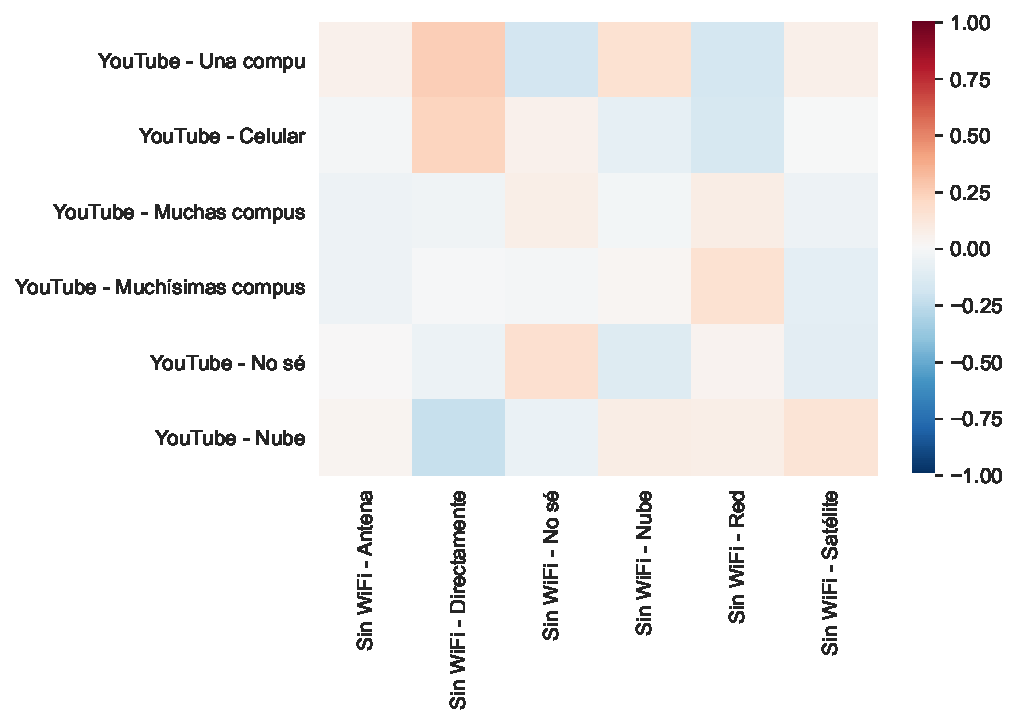
\includegraphics[width=0.65\textwidth]{images_analisis/30.pdf}
    \caption{Relación entre las respuestas a las preguntas ``\textit{YouTube}'' y ``\textit{Mensajes sin WiFi}''.}
    \label{fig:analisis30}
\end{figure}

A su vez, parecería que ``\textit{YouTube - Nube}'' y ``\textit{Sin WiFi - Directamente}'' están correlacionadas negativamente.

Como estamos utilizando variables binarias, decidimos probar para los pares de preguntas que parecían mostrar una mayor correlación con el método de \textit{chi cuadrado}, ya que este es más adecuado para este tipo de variables.

Lo que intentamos es rechazar la hipótesis nula, que en nuestro caso es que dos respuestas dadas son independientes. 

Utilizamos una implementación de \textit{chi cuadrado} de la librería de \textit{Python} \texttt{numpy}, y para ello, en primer lugar realizamos las tablas de correlación de cada par, que muestran cuántos alumnos y alumnas eligieron una, las dos, o ninguna de las respuestas. 

El resultado de la tabla de correlación se puede leer en las tablas expuestas a continuación, que se interpretan de la siguiente manera:

\begin{itemize}
    \item La celda (0,0) en la fila donde se indica “observado'' muestra cuántos alumnos o alumnas no eligieron ninguna de las dos respuestas.
    \item Las celdas (0,1) y (1,0)  en la fila donde se indica “observado'' muestra cuántos alumnos o alumnas eligieron alguna de las dos respuestas.
    \item La celda (1,1), en la fila donde se indica “observado'' muestra cuántos alumnos o alumnas eligieron ambas respuestas.

\end{itemize}

El valor de la fila donde se indica ``esperado'' es el valor que, suponiendo que las respuestas son independientes, deberíamos esperar para esa combinación de respuestas elegidas. Este valor es calculado por el algoritmo \texttt{chi2\_contingency} mencionado anteriormente, pero es interesante presentarlo ya que nos ayudará a interpretar el resultado. Si observo algo que es parecido a lo que esperaba observar (es decir, el ``observado'' es parecido al ``esperado'') entonces no puedo rechazar la hipótesis de que sean variables independientes.

El resultado de realizar el método de chi cuadrado es el p-valor. Un p-valor cercano a 1 no nos permite rechazar la hipótesis nula, es decir, no se puede afirmar que las dos respuestas no sean independientes. Por el contrario, un p-valor cercano a 0 quiere decir que es poco probable observar lo “observado” si las variables son independientes, es decir que podrían estar relacionadas. 

Veamos ahora los resultados para los distintos pares de preguntas comentados previamente.

En la Fig. \ref{fig:analisis32} podemos ver que las respuestas ``\textit{Mandar - copia}'' y ``\textit{Borrar - No puedo}'' parecerían estar altamente correlacionadas, ya que el p-valor obtenido es menor a 0,0001. Este resultado es muy favorable ya que indica que una de las combinaciones de respuestas más frecuentes es de hecho una combinación sin \textit{misconceptions}. Sin embargo, como podemos ver en el campo ``\textit{observado}'', 41 de los chicos (es decir un 28,47\% del total) eligieron estas dos respuestas simultáneamente.

\begin{figure}[h]
    \centering
    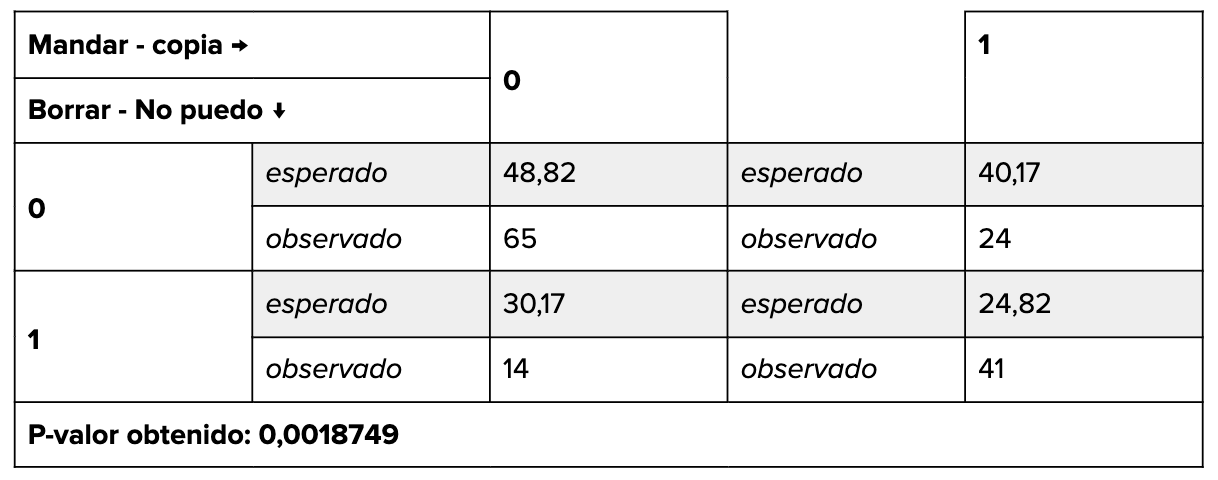
\includegraphics[width=0.65\textwidth]{images_analisis/32.png}
    \caption{Relación entre ``\textit{Mandar - copia}'' y ``\textit{Borrar - No puedo}''}
    \label{fig:analisis32}
\end{figure}

\newpage

Otra observación interesante surge de la Fig. \ref{fig:analisis33}. En esta podemos ver que 38 alumnos (26,38\% del total) eligieron al mismo tiempo las respuestas ``\textit{Mandar - En WhatsApp}'' y ``\textit{Borrar - En el chat}''. El p-valor obtenido al utilizar el método de chi cuadrado corrobora que entre ambas respuestas hay una correlación. Y justamente, estas dos respuestas dan a pensar en la idea de que la información compartida a través de WhatsApp es almacenada de alguna manera ``\textit{remotamente}'' en los servidores del servicio de mensajería, y que no se genera una copia local para la persona a la cual se le compartieron los datos enviados.  

\begin{figure}[h]
    \centering
    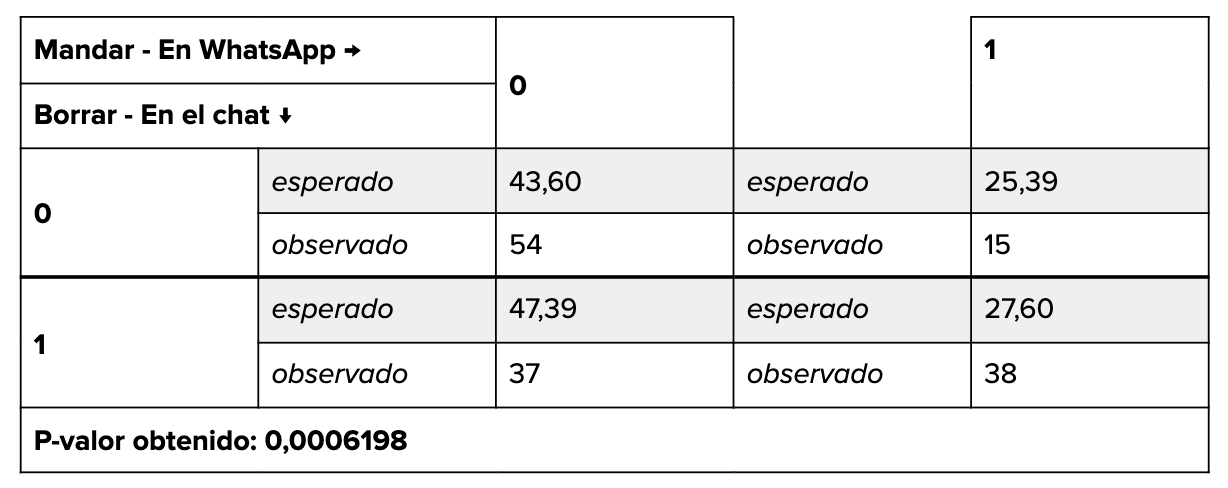
\includegraphics[width=0.65\textwidth]{images_analisis/33.png}
    \caption{Relación entre ``\textit{Mandar - En WhatsApp}'' y ``\textit{Borrar - En el chat}''}
    \label{fig:analisis33}
\end{figure}

En la Fig. \ref{fig:analisis34} observamos que existe correlación entre las respuestas ``\textit{Sin WiFi - Directamente}'' y ``\textit{YouTube - Una compu}''. Esta relación podría interpretarse tal vez como la falta de una noción de la infraestructura subyacente en las tecnologías sobre las que indagamos: por un lado, en la pregunta sobre cómo viajan los mensajes cuando no hay WiFi se responde que los mensajes viajan ``\textit{directamente}'', sin considerar la red sobre la cual se apoya la telefonía móvil. Por otro lado, al responder que los videos en YouTube se almacenan en una única compu queda evidenciado la \textit{misconception} respecto de la cantidad de información de la que hablamos y de la infraestructura necesaria para su almacenamiento.

\begin{figure}[h]
    \centering
    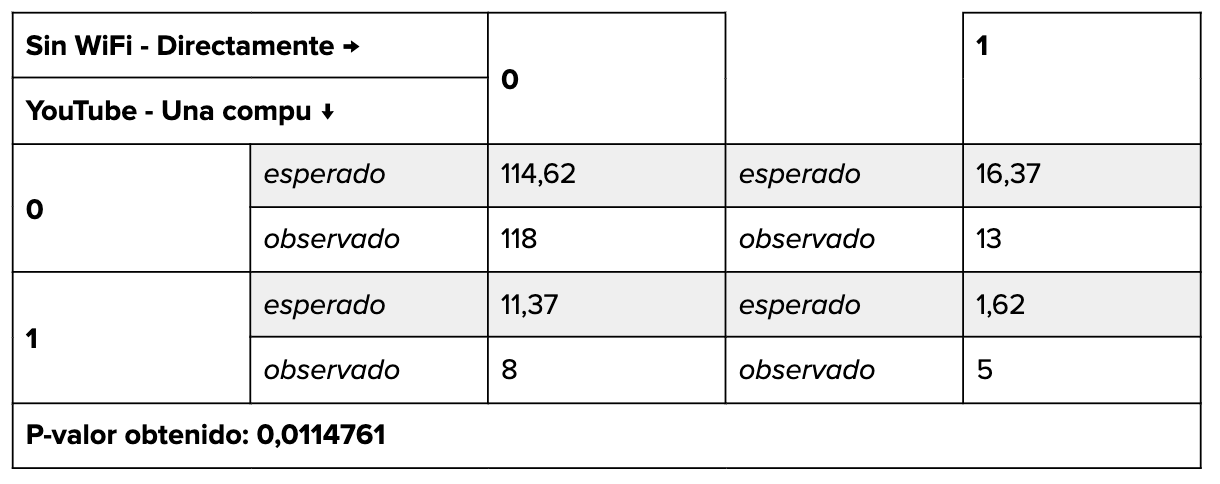
\includegraphics[width=0.65\textwidth]{images_analisis/34.png}
    \caption{Relación entre ``\textit{Sin WiFi - Directamente}'' y ``\textit{YouTube - Una compu}''}
    \label{fig:analisis34}
\end{figure}

\newpage

Una reflexión similar a la anterior podemos hacer con los resultados analizados en la Fig. \ref{fig:analisis35}, en la que vemos que las respuestas ``\textit{Sin WiFi - Directamente}'' y ``\textit{YouTube - Celular}'' se encuentran también relacionadas, pero esta vez, profundizando aún más la \textit{misconception} acerca del volumen de datos que se maneja en YouTube, al responder que los videos se almacenan en ``\textit{un celular}''.

\begin{figure}[h]
    \centering
    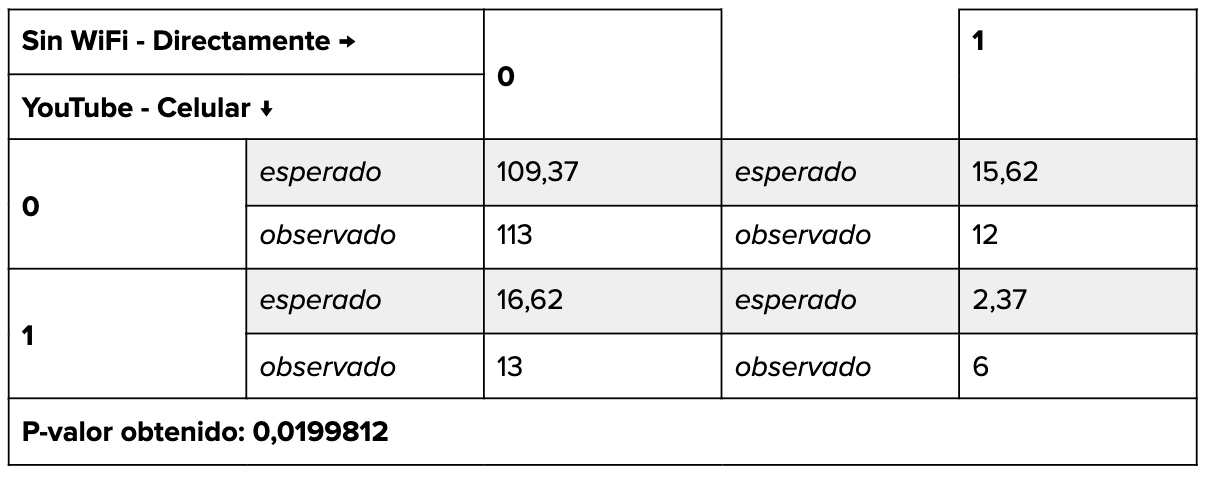
\includegraphics[width=0.65\textwidth]{images_analisis/35.png}
    \caption{Relación entre ``\textit{Sin WiFi - Directamente}'' y ``\textit{YouTube - Celular}''}
    \label{fig:analisis35}
\end{figure}

Adicionalmente, probamos utilizando el método de \textit{clustering aglomerativo}. Con esta técnica se generan \textit{clusters} con los grupos de preguntas más similares, considerando los chicos que respondieron con o sin \textit{misconception}.

El gráfico que se genera se interpreta de la siguiente manera: cada fila representa a un alumno o alumna y cada columna, a una de las preguntas que les propusimos. Cada celda generada se encuentra coloreada en verde oscuro si se respondió con una \textit{misconception} o sin colorear si se respondió sin \textit{misconception}. El algoritmo reordena las filas y columnas de manera de poder visualizar mejor los \textit{clusters} generados, es decir, las preguntas para las cuales se respondió más similarmente. A su vez, produce un dendrograma que muestra los vínculos entre los grupos obtenidos de manera jerárquica. 

En nuestro caso, como se observa en la Fig. \ref{fig:analisis31}, confirmamos que las preguntas más similares son, por un lado, ``\textit{Mandar Fotos}'' y ``\textit{Borrar Fotos}'' y, a su vez, éstas forman un cluster con ``\textit{Gratuidad Apps}''. Por otro lado, la pregunta ``\textit{YouTube}'' y ``\textit{Mensajes sin WiFi}'' forman otro \textit{cluster}.

Es interesante destacar que al utilizar este método visualizamos también cuál es la pregunta que menos se relaciona con las demás. En este caso es ``\textit{Acceso Fotos}''. Un posible motivo por el cuál puede pasar esto es que ésta era una pregunta que, si bien pertenecía al grupo de preguntas sobre el envío de fotos por WhatsApp, su respuesta correcta era bastante accesible al sentido común de los alumnos, y por lo tanto no termina siendo un indicador de si poseen o no \textit{misconceptions} respecto a este tema o a los demás.

\begin{figure}[h]
    \centering
    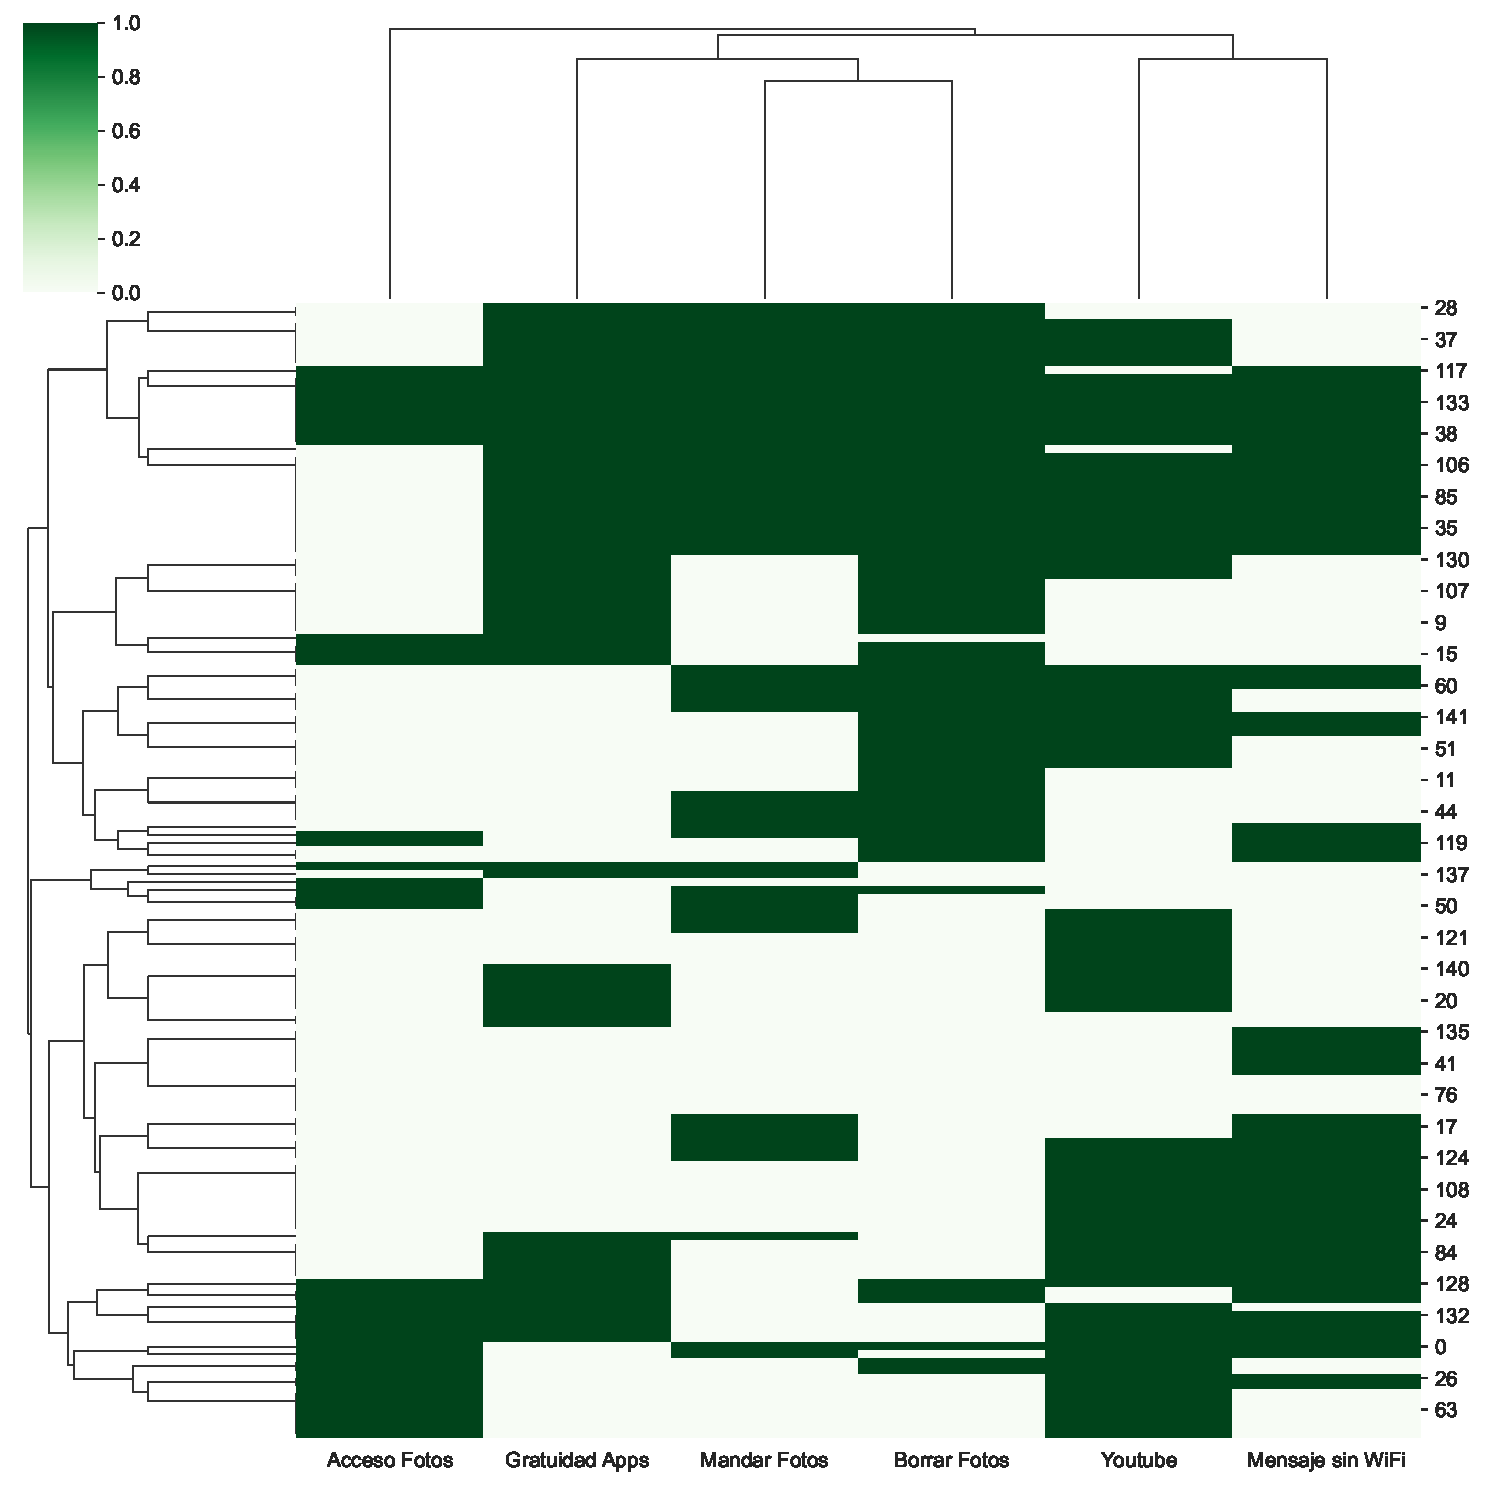
\includegraphics[width=1\textwidth]{images_analisis/31.pdf}
    \caption{\textit{Clustermap} que representa cuáles son las preguntas más relacionadas en función de las respuestas de los alumnos.   }
    \label{fig:analisis31}
\end{figure}